% KAPITEL 4: Auswertung und Diskussion (04_ergebnisteil.tex)


\section{Auswertung und Diskussion}
\label{sec:auswertung_diskussion}

Dieses Kapitel widmet sich der detaillierten Evaluation, wie unterschiedliche Leitergeometrien die Messgenauigkeit von Stromwandlern beeinflussen. Im Zentrum steht die Analyse, in welchem Maße die räumliche Anordnung der Primärleiter \gls{sym:I_p} über magnetische Streufelder, Feldüberlagerungen und daraus resultierende Sättigungseffekte des Eisenkerns die Fehlerkennlinien der Prüflinge verändert. 



Die Auswertung basiert auf den erfassten Messreihen über den gesamten Lastbereich — von der Teillast bei \SI{5}{\percent} bis zum Überstrom bei \SI{120}{\percent} — und stellt die Ergebnisse der konventionellen Parallelanordnung sowie der feldoptimierten Dreieckskonfiguration systematisch gegenüber.

Zunächst wird der Geometrieeinfluss über alle Prüflinge hinweg qualitativ und quantitativ eingeordnet, um allgemeine Trends und wiederkehrende Muster, wie etwa eine erhöhte Empfindlichkeit des mittleren Leiters in der Parallelanordnung, zu identifizieren. Darauf aufbauend werden die Ergebnisse modell- und phasenspezifisch analysiert. Hierbei wird insbesondere bewertet, ob die beobachteten Abweichungen \gls{sym:epsilon} primär durch interferierende Magnetfelder benachbarter Leiter oder durch eine konstruktiv bedingte Begrenzung des magnetischen Kreises, beispielsweise ein geringes Kernvolumen, verursacht werden. 



Ergänzend werden die Differenzen zwischen Standardwandlern, kompensierten Systemen sowie der \gls{ffp}-Technologie diskutiert, um die Wirksamkeit von Schirmmaßnahmen im Kontext realistischer Leitergeometrien validieren zu können.

Im abschließenden Teil dieses Kapitels folgt eine ökonomische Bewertung der Resultate. Dazu werden die Konfigurationen nicht nur hinsichtlich der normativen Einhaltung der Genauigkeitsklasse \num{1}, sondern auch nach ihrem operativen Mehrwert (Messgüte im relevanten Betriebsbereich) und dem konstruktiven Aufwand gegenübergestellt. Der Aufwand umfasst dabei Aspekte wie die Geometrieänderung der Schienen, die Bürdenanpassung sowie die gezielte Wahl der Wandlertechnologie. Ziel ist es, aus den Messergebnissen belastbare Empfehlungen abzuleiten, welche Leiteranordnung und welches Wandlerkonzept unter Berücksichtigung technischer und wirtschaftlicher Randbedingungen zu bevorzugen sind.



\subsection{Einfluss der Leitergeometrie auf die Messgenauigkeit}
\label{sec:einfluss_leitergeometrie}

Die folgenden Diagramme visualisieren die Übersetzungsmessabweichungen \gls{sym:epsilon} der Stromwandler in Abhängigkeit vom Primärstrom \gls{sym:I_p} sowie der gewählten Leiteranordnung. Der Vergleich erfolgt jeweils zwischen Wandlern mit identischem Bemessungsstrom \gls{sym:In}. Eine detaillierte Beschreibung der konstruktiven Umsetzung dieser Leiteranordnungen findet sich in Abschnitt \ref{sec:layout_geometrie}.



Zur eindeutigen visuellen Differenzierung der Konfigurationen gelten in den Diagrammen folgende Konventionen:

\begin{itemize}
    \item \textbf{Parallelanordnung:} Diese Referenzkonfiguration wird durch eine durchgezogene Linie in Kombination mit Kreismarkern dargestellt.
    \item \textbf{Dreieckskonfiguration:} Diese feldoptimierte Anordnung ist durch eine gestrichelte Linie sowie Dreieckssymbole gekennzeichnet.
    \item \textbf{Farbgebung:} Die Farben sind spezifischen Wandlermodellen fest zugeordnet und verbleiben über beide Anordnungen hinweg identisch, um einen unmittelbaren Vergleich der Kennlinienverläufe zu gewährleisten.
\end{itemize}



Diese systematische Darstellungsweise erlaubt die direkte Bewertung des Geometrieeinflusses auf den jeweiligen Wandlertyp sowie die Identifikation technologischer Vorteile — beispielsweise durch die \gls{ffp}-Technologie oder den Einsatz von Kompensationswicklungen — unter variierenden magnetischen Feldbedingungen.



\subsubsection{Referenzanalyse bei \SI{2000}{A}: Einfluss der Leitergeometrie auf verschiedene Wandlerkonzepte}
\label{sec:analyse_messreihe_2000A}

Die Untersuchung der Stromwandler bei einem Nennstrom \gls{sym:In} von \SI{2000}{A} liefert differenzierte Ergebnisse für die verschiedenen Modelle und Leiteranordnungen. Abbildung~\ref{dia:2000A_zusammenfassung} stellt die Verläufe der vier Prüflinge gegenüber und verdeutlicht die Einhaltung der Genauigkeitsklasse \num{1} für den Großteil der Messpunkte. Der grafische Vergleich hebt hervor, dass insbesondere zwei Konfigurationen erkennbare Abweichungen aufweisen. Dies betrifft den \textit{Redur~13A1030.ffp} in der Dreieckskonfiguration sowie den \textit{Celsa~ALO~10030} in der Parallelanordnung. Beide Wandler verlassen in diesen spezifischen Szenarien die vorgegebenen Toleranzbereiche.



\begin{diagram}[H]
    \centering
    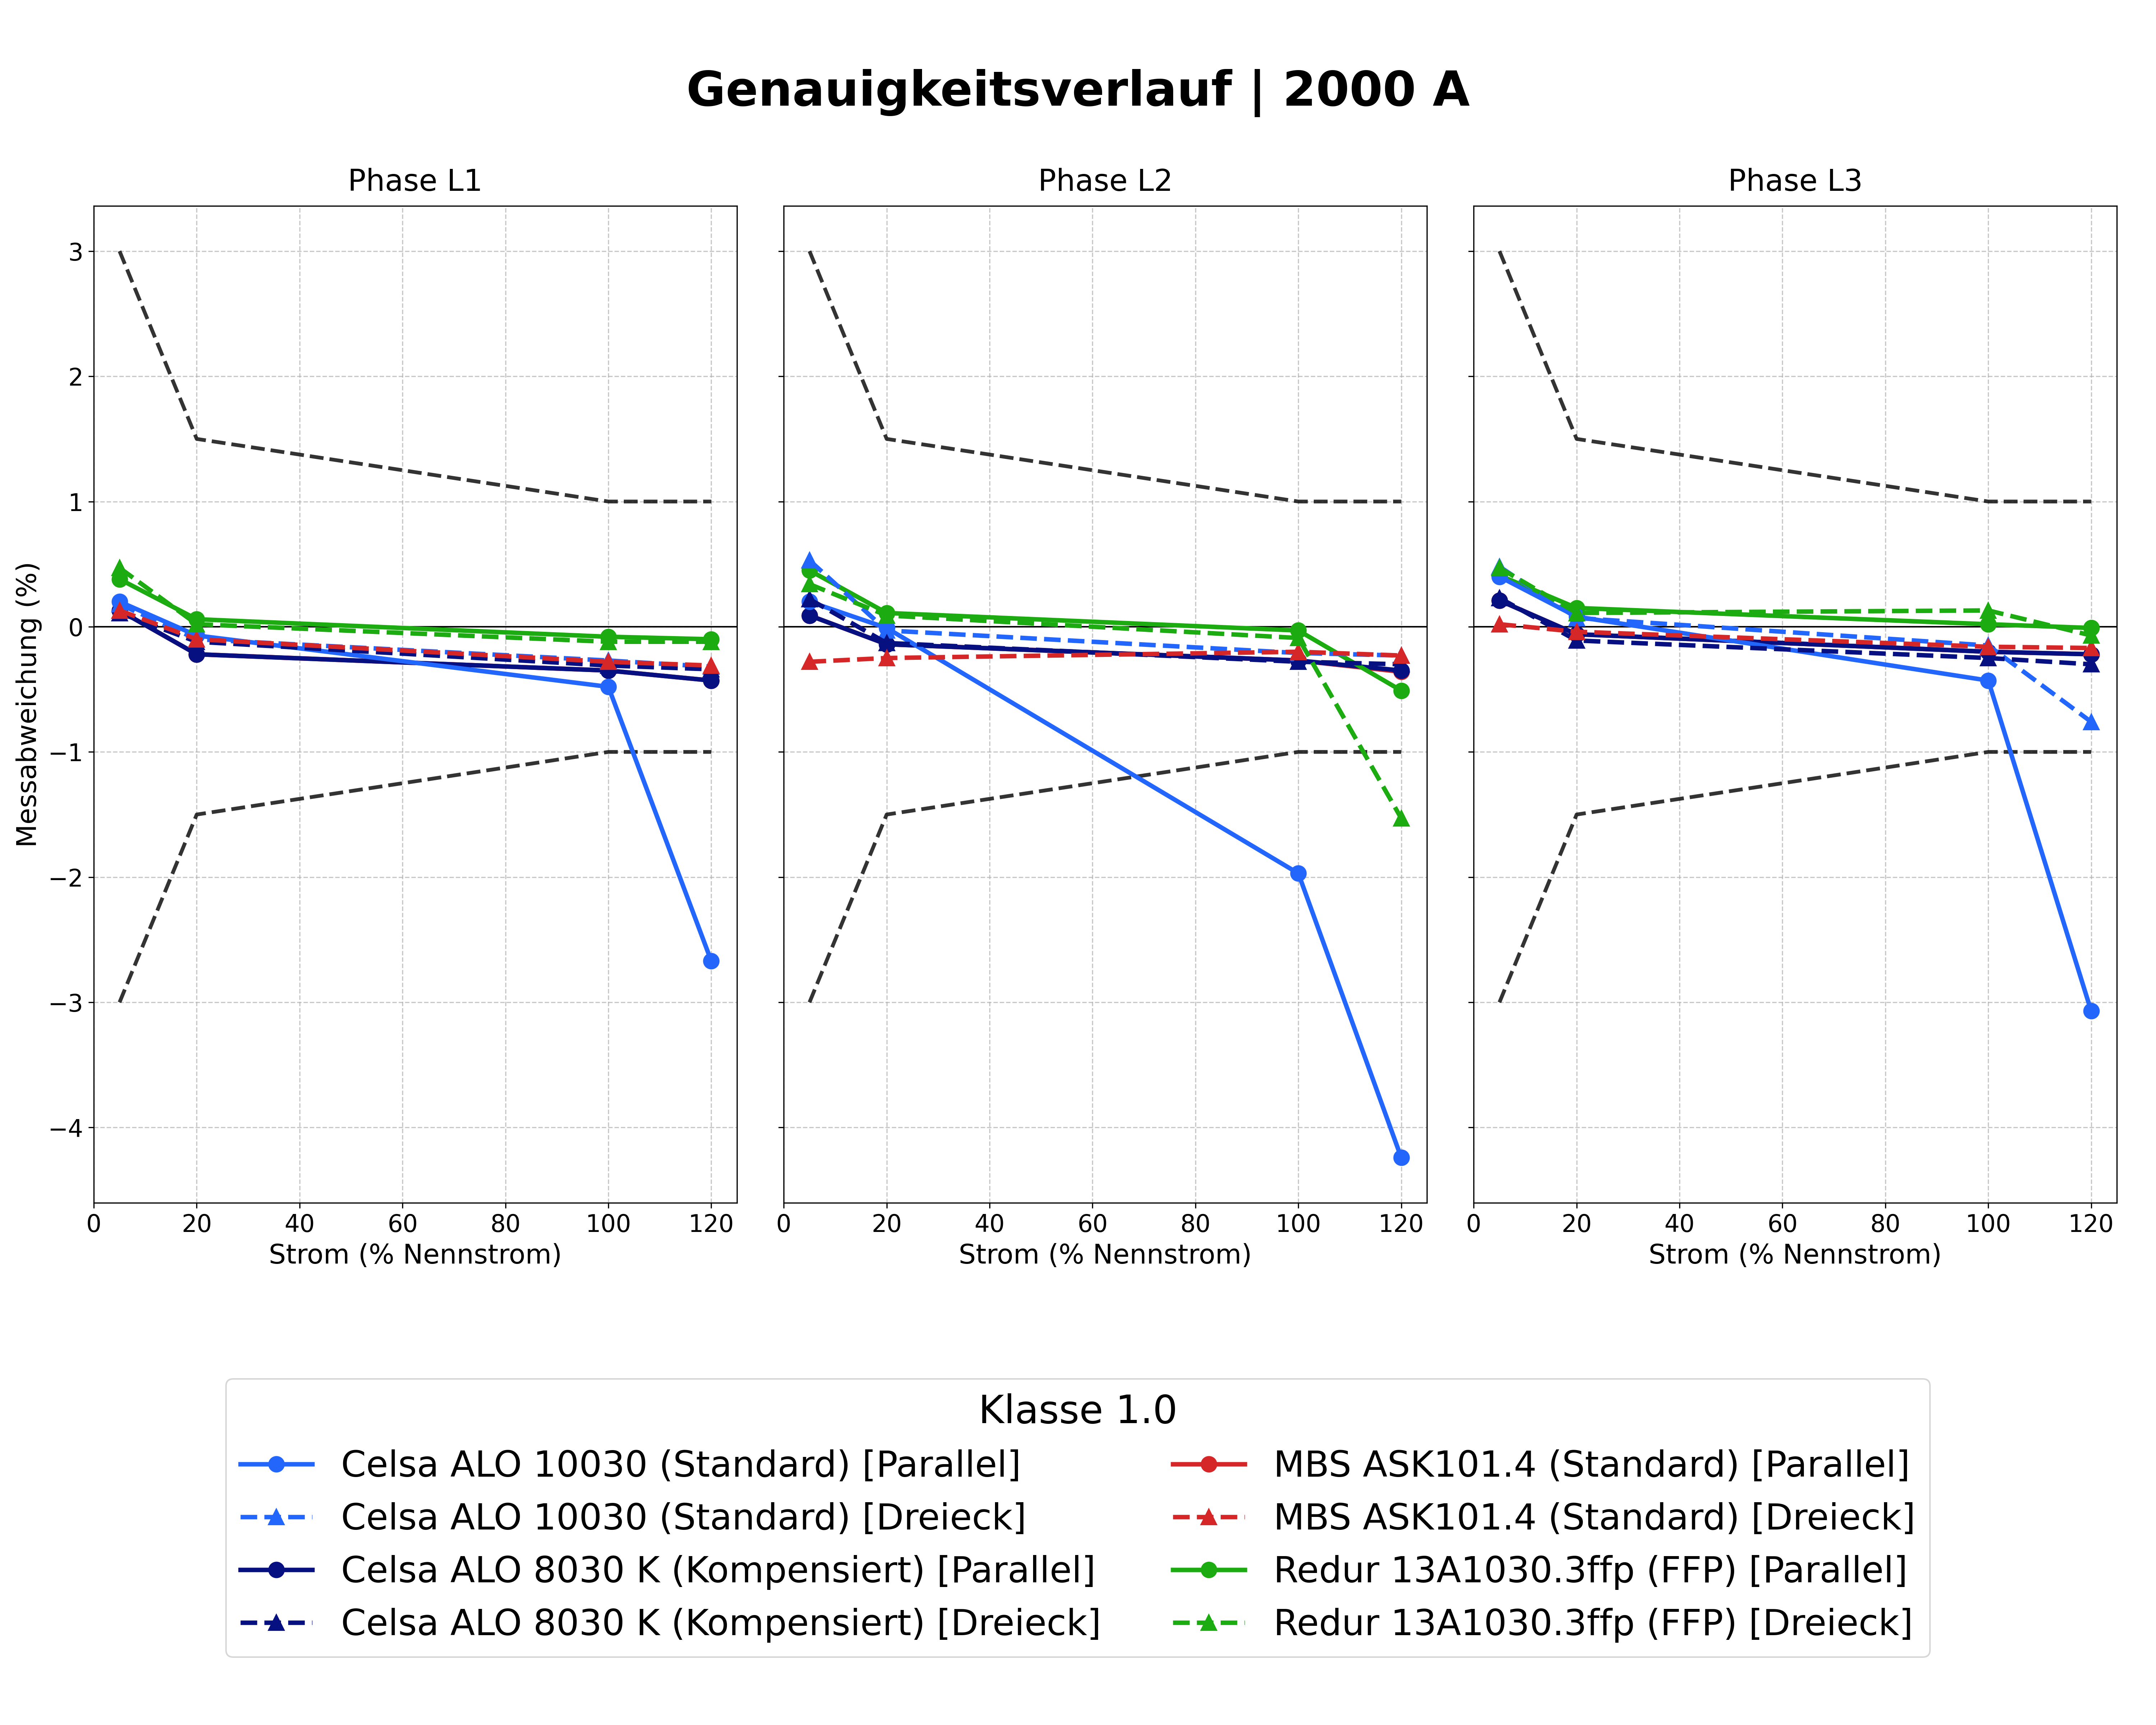
\includegraphics[width=1.0\textwidth]{03_Ressourcen/dia_neu/verlauf/mes_2000A_verlauf.png}
    \caption{Zusammenfassender Vergleich der Leitergeometrien bei \SI{2000}{A}}
    \label{dia:2000A_zusammenfassung}
\end{diagram}

Eine bauliche Besonderheit weist der \textit{Redur~13A1030.ffp} auf. Wie in Abbildung~\ref{fig:wandler_fremdfeldprotektor} zu erkennen ist, befinden sich die Fremdfeldprotektoren (\gls{ffp}) an den seitlichen Flanken des Gehäuses. Diese Positionierung schirmt den Eisenkern gegen magnetische Streufelder benachbarter Leiter ab, sofern diese seitlich angeordnet sind. In der parallelen Leiterführung resultiert dies in normkonformen Messergebnissen, da die Beeinflussung durch die Nachbarphasen minimiert wird.



\begin{figure}[H]
    \centering
    \includegraphics[width=1.0\textwidth]{03_Ressourcen/Bilder/wandler_redur_2000A_dreiecksmessung_beschriftet.pdf}
    \caption{Seitliche Fremdfeldprotektoren am \textit{Redur~Wandler}}
    \label{fig:wandler_fremdfeldprotektor}
\end{figure}

Die Grenzen dieser Schirmungstechnologie offenbaren sich in der Dreieckskonfiguration. Die detaillierten numerischen Ergebnisse für diesen Aufbau sind in Tabelle~\ref{tab:messergebnisse_redur_2000A} im Anhang zu finden. Die Phase L2 weist bei \SI{120}{\percent} des Nennstroms eine Übersetzungsmessabweichung \gls{sym:epsilon} von \num{-1,50}\,\% auf. Dieser Wert liegt außerhalb der zulässigen Toleranz der Genauigkeitsklasse \num{1}. Ursächlich hierfür ist die fehlende magnetische Schirmung auf der Rückseite des Wandlergehäuses. In der Dreiecksgeometrie können die Magnetfelder der benachbarten Leiter an dieser ungeschützten Stelle in den Eisenkern eindringen und diesen partiell sättigen. Im Gegensatz dazu bleibt die Phase L1 mit einer Abweichung von lediglich \num{-0,10}\,\% im selben Lastpunkt weit innerhalb der Normgrenzen.

Ein konträres Verhalten ist beim Modell \textit{Celsa~ALO~10030} zu beobachten. Tabelle~\ref{tab:messergebnisse_celsa_2000A} im Anhang dokumentiert die Messergebnisse für diesen Wandler und belegt substanzielle Einbußen der Genauigkeit in der parallelen Leiteranordnung. Bereits bei Nennstrom \gls{sym:In} verletzt die Phase L2 mit \num{-2,00}\,\% den zulässigen Grenzwert. Bei einer Überlast von \SI{120}{\percent} steigt die Abweichung \gls{sym:epsilon} weiter auf \num{-4,20}\,\% an. Auch die Außenleiter L1 und L3 zeigen in der Parallelanordnung bei \SI{120}{\percent} Last mit Werten von \num{-2,70}\,\% beziehungsweise \num{-3,10}\,\% erkennbare Fehler. Die Änderung der Geometrie hin zur Dreiecksanordnung bewirkt bei diesem Modell eine Verbesserung: Der Fehler der Phase L2 reduziert sich hierbei bei \SI{120}{\percent} Last auf einen unkritischen Wert von \num{-0,20}\,\%.

Diese Abhängigkeit des Fehlers vom Primärstrom \gls{sym:I_p} wird in Abbildung~\ref{dia:2000A_celsa_zusammenfassung} grafisch aufbereitet. Das Diagramm veranschaulicht den steilen Abfall der Messkurven für die Parallelanordnung ab etwa \SI{20}{\percent} des Nennstroms. Im Vergleich dazu verlaufen die Kurven der Dreiecksanordnung weitestgehend linear und verbleiben im Toleranzbereich.

\begin{diagram}[H]
    \centering
    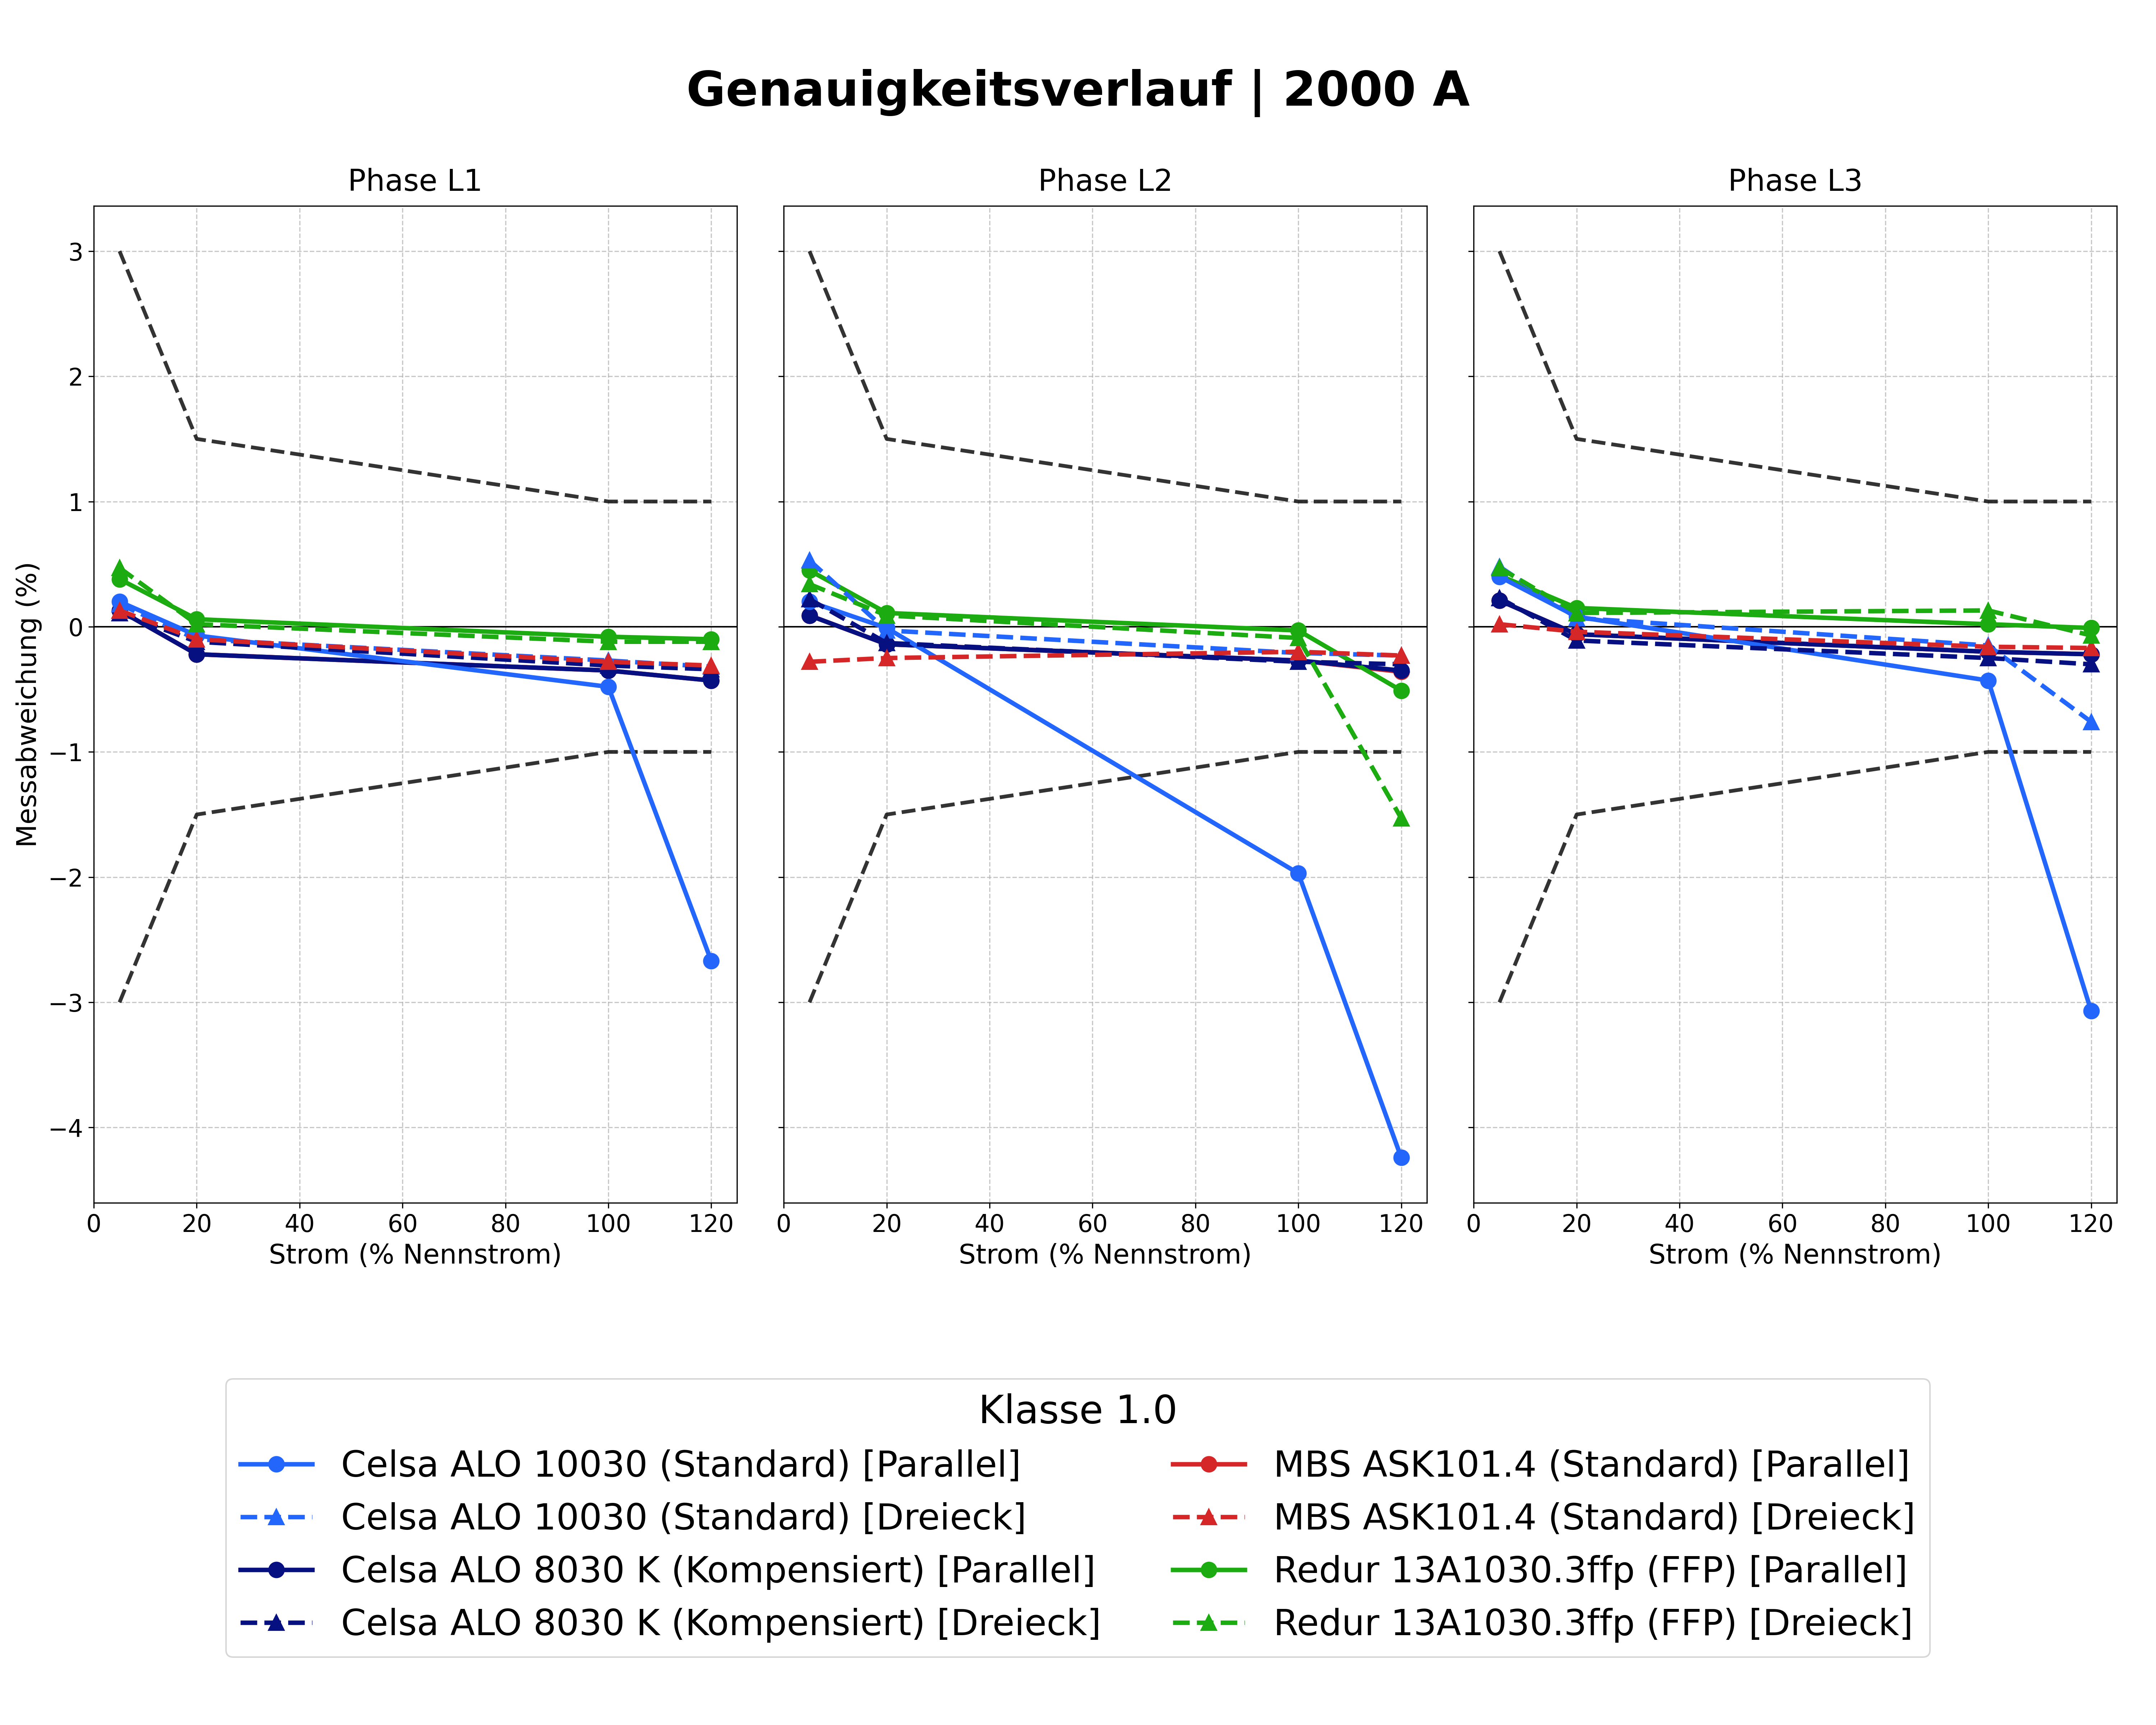
\includegraphics[width=1.0\textwidth]{03_Ressourcen/dia_neu/verlauf/mes_2000A_verlauf.png}
    \caption{Messfehlerverlauf des \textit{Celsa~ALO~10030} in Abhängigkeit vom Primärstrom \gls{sym:I_p}}
    \label{dia:2000A_celsa_zusammenfassung}
\end{diagram}

Im Gegensatz zu den Abweichungen der vorangegangenen Modelle zeigen der \textit{Celsa~ALO~8030~K} und der \textit{MBS~ASK~101.4} eine hohe Stabilität gegenüber externen Feldern. Diese Unempfindlichkeit lässt sich beim \textit{Celsa~ALO~8030~K} auf die Bauweise als kompensierter Wandler zurückführen, wie in Abschnitt \ref{sec:kompensationswicklungen} erläutert wird. Tabelle~\ref{tab:messergebnisse_celsa8030_2000A} im Anhang fasst die Ergebnisse für dieses Modell zusammen. Selbst unter Volllast und Überstrom bleiben alle Phasen in beiden geometrischen Anordnungen sicher innerhalb der Klasse \num{1}. Die maximale Abweichung tritt in der Parallelanordnung bei Phase L1 mit einem Wert von \num{-0,40}\,\% auf.

Ein ähnlich robustes Verhalten bestätigt Tabelle~\ref{tab:messergebnisse_mbs_2000A} im Anhang für den \textit{MBS~ASK~101.4}. Auch hier sind keine signifikanten Einflüsse durch die Leiteranordnung erkennbar. Die Messwerte liegen konstant auf einem Niveau vergleichbar mit dem \textit{Celsa~ALO~8030~K}. In der Dreiecksanordnung erreicht die Phase L1 bei \SI{120}{\percent} Last beispielsweise eine Abweichung von \num{-0,30}\,\% und demonstriert damit die Unempfindlichkeit dieses Modells gegenüber den untersuchten geometrischen Anordnungen.

\subsubsection{Einfluss der Leitergeometrie auf das Sättigungsverhalten bei \SI{2500}{A}}
\label{sec:analyse_messreihe_2500A}

Die Analyse der Messreihe bei einem Nennstrom \gls{sym:In} von \SI{2500}{A} verdeutlicht den massiven Einfluss der Leitergeometrie auf unterschiedliche Wandlertechnologien. Im Fokus steht der Vergleich zwischen dem kompensierten Wandler \textit{Celsa~ALO~10050~K} und dem Standardwandler \textit{Celsa~ALO~10030} in Bezug auf ihre Stabilität in Parallel- und Dreieckskonfigurationen.



\begin{aufgabenbox}
    Hier möchte ich noch eine Simulation machen.
    Es sollen die Sättigungseffekte des Eisenkernes betrachtet werden.
\end{aufgabenbox}



\begin{diagram}[H]
    \centering
    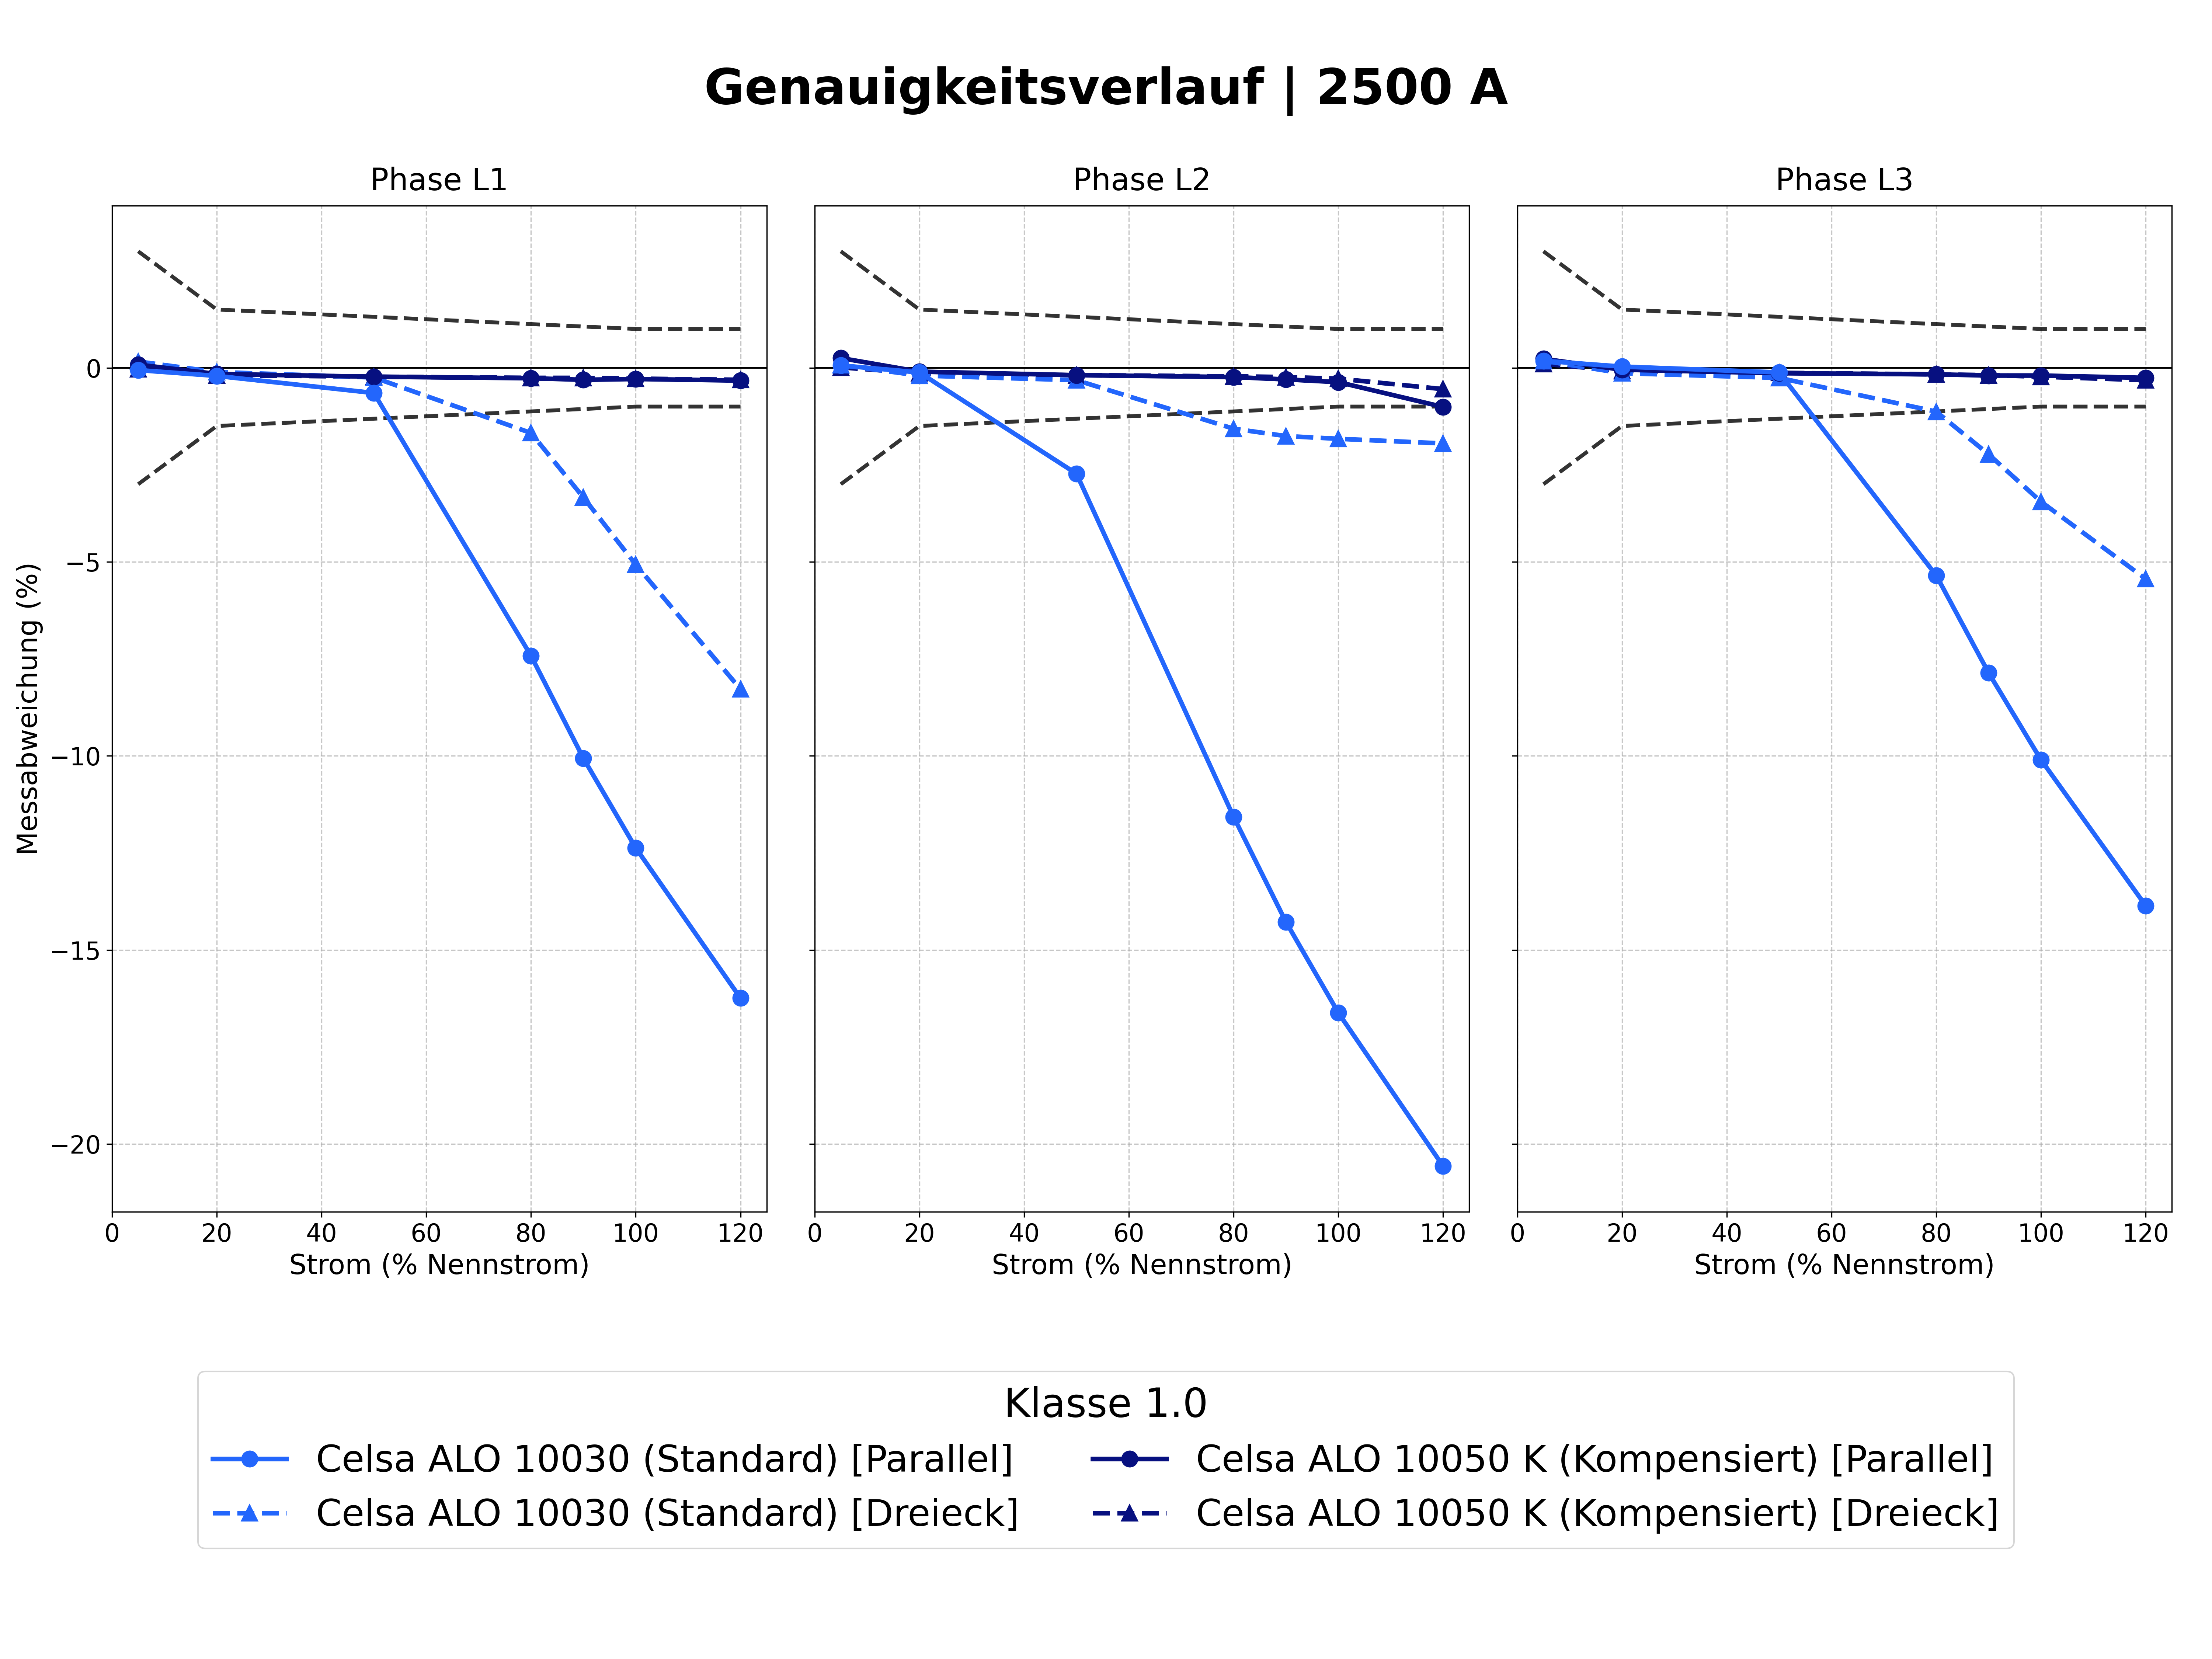
\includegraphics[width=1.0\textwidth]{03_Ressourcen/dia_neu/verlauf/mes_2500A_verlauf.png}
    \caption{Zusammenfassender Vergleich der Leitergeometrien bei \SI{2500}{A}}
    \label{dia:2500A_zusammenfassung}
\end{diagram}

Die Messergebnisse des kompensierten Wandlers \textit{Celsa~ALO~10050~K} belegen, dass dieser über den Großteil des Messbereichs eine hohe Genauigkeit aufweist (siehe Tabelle~\ref{tab:messergebnisse_celsa10050_2500A_alle} im Anhang). In der Parallelanordnung bewegt sich der Wandler nahezu durchgehend innerhalb der normativen Vorgaben. Eine Ausnahme bildet die Phase L2 im Überlastbereich bei \SI{120}{\percent} Nennstrom \gls{sym:In}. Hier überschreitet der Wandler den Grenzwert mit einer Übersetzungsmessabweichung \gls{sym:epsilon} von rund \num{-1,00}\,\% knapp, was einem absoluten Fehlstrom von circa \num{30,00}\,\unit{A} entspricht. 

In der Dreieckskonfiguration reduziert sich dieser Messfehler auf etwa \num{-0,55}\,\%, wodurch die normative Genauigkeitsklasse \num{1} wieder eingehalten wird. Dies verdeutlicht, dass selbst ein kompensierter Wandler nicht vollständig immun gegen externe Magnetfelder ist, die Auswirkungen jedoch im Vergleich zur Standardtechnologie gering bleiben. Da sich der Fehlerbetrag hierbei fast halbiert, führt die Dreiecksgeometrie in diesem kritischen Lastpunkt zu einer annähernden Verdopplung der Messgenauigkeit.



Im Gegensatz dazu zeigt der nicht kompensierte Standardwandler \textit{Celsa~ALO~10030} in beiden Anordnungen erhebliche Abweichungen, die auf eine beginnende magnetische Sättigung hindeuten (siehe Tabelle~\ref{tab:messergebnisse_celsa10030_2500A_alle} im Anhang). In der Parallelanordnung steigt der Fehler bereits ab \SI{50}{\percent} Nennstrom \gls{sym:In} erkennbar an. Bei \SI{100}{\percent} Last liegen die Abweichungen \gls{sym:epsilon} zwischen \num{-10,00}\,\% und \num{-16,00}\,\%. Um das Ausmaß dieser Sättigungseffekte im Hochlastbereich zu verdeutlichen, stellt Tabelle~\ref{tab:vergleich_hochstlast_celsa_extended} die absoluten Fehlströme der Phase L2 gegenüber und quantifiziert den Präzisionsgewinn durch die geometrische Optimierung.

\begin{table}[H]
    \centering
    \caption{Vergleich der Fehlströme und Genauigkeitsgewinn (\textit{Celsa~ALO~10030}, Phase L2)}
    \label{tab:vergleich_hochstlast_celsa_extended}
    \small
    \begin{tabular}{l S[table-format=4.0] S[table-format=2.2] S[table-format=3.2] S[table-format=2.2]}
        \toprule
        {Lastpunkt}  & {Primärstrom \gls{sym:I_p}} & {Fehlstrom Dreieck} & {Fehlstrom Parallel} & {Verbesserung} \\
        {[\% \gls{sym:In}]} & {[\unit{A}]}         & {[\unit{A}]}               & {[\unit{A}]}                & {[\unit{\%}]}         \\
        \midrule
        80           & 2000          & 31.35               & 231.42               & 10.00           \\
        90           & 2250          & 39.67               & 321.22               & 12.50           \\
        100          & 2500          & 45.85               & 415.59               & 14.80           \\
        120          & 3000          & 58.49               & 616.96               & 18.60           \\
        \bottomrule
    \end{tabular}
\end{table}

Wie den Werten zu entnehmen ist, bricht die Genauigkeit im Überlastbereich bei \SI{120}{\percent} drastisch ein. Während in der Parallelanordnung ein Fehlstrom von über \num{616,96}\,\unit{A} auftritt, sinkt dieser in der Dreieckskonfiguration auf rund \num{58,49}\,\unit{A}. Dies entspricht einer Verbesserung der Genauigkeit um \num{18,60} Prozentpunkte. Auch die Phasen L1 und L3 liegen in der Parallelanordnung mit \num{-16,20}\,\% beziehungsweise \num{-13,90}\,\% weit außerhalb der Toleranzgrenzen, profitieren jedoch in ähnlichem Maße von der Umstellung auf die Dreiecksgeometrie.

Dennoch muss konstatiert werden, dass selbst die optimierte Dreiecksanordnung nicht ausreicht, um die normativen Vorgaben zu erfüllen. Trotz der Fehlerminimierung verbleibt der Wandler außerhalb der Genauigkeitsklasse \num{1}. Diese verbleibende Abweichung deutet auf eine grundsätzliche Unterdimensionierung des magnetischen Kreises hin. Ein Vergleich mit den Ergebnissen aus Abschnitt \ref{sec:analyse_messreihe_2000A} stützt diese Hypothese, da bereits dort dieser Wandlertyp Sättigungstendenzen im Nennstrombereich zeigte. Bei dem hier untersuchten \SI{2500}{A}-Modell wird anhand von Tabelle~\ref{tab:vergleich_hochstlast_celsa_extended} ersichtlich, dass der massive Fehleranstieg bereits bei \SI{80}{\percent} der Nennlast einsetzt, was einem Primärstrom \gls{sym:I_p} von \SI{2000}{A} entspricht.

Damit korreliert der Sättigungsbeginn exakt mit den Beobachtungen der vorherigen Messreihe. Dies lässt den Schluss zu, dass das physikalische Eisenkernvolumen dieses Bauteils unabhängig von der Nennstromangabe auf dem Typenschild für Ströme oberhalb von \SI{2000}{A} nicht ausreichend dimensioniert ist. Dieser empirische Befund bestätigt die theoretischen Zusammenhänge, die durch Gleichung \ref{eq:b_phi_relation} beschrieben werden. Wie dort hergeleitet, führt der geringe Eisenquerschnitt \gls{sym:A} dazu, dass sich der magnetische Fluss auf eine zu kleine Fläche konzentriert. Dies bewirkt trotz der absolut gesehen geringeren Störflussaufnahme einen kritischen Anstieg der resultierenden Flussdichte \gls{sym:B_res}, wodurch die Sättigungsgrenze des Materials frühzeitig erreicht wird.

Tabelle~\ref{tab:wandler_volumen} untermauert diese Vermutung durch die Berechnung des effektiven Materialvolumens. Während der Typ \textit{Celsa~ALO~10050~K} über ein berechnetes Nettovolumen von \num{623,60}\,\unit{cm^3} verfügt, weist der hier betrachtete \textit{Celsa~ALO~10030} lediglich \num{265,50}\,\unit{cm^3} auf. Damit steht diesem Wandler weniger als die Hälfte des Volumens zur Verfügung, was die frühzeitige Sättigung physikalisch plausibilisiert.

\begin{table}[H]
    \centering
    \caption{Berechnetes Nettovolumen der untersuchten Wandler}
    \label{tab:wandler_volumen}
    \begin{tabular}{l c c S[table-format=3.2]}
        \toprule
        {Modell}    & {Gehäusemaße ($H \times B \times T$)} & {Fenstergeometrie}        & {Nettovolumen [\unit{cm^3}]} \\
        \midrule
        \textit{Celsa~ALO~10030}   & $31 \times 129 \times \SI{141}{mm}$   & $\varnothing$ \SI{55}{mm} & 265.50                        \\
        \textit{Celsa~ALO~10050~K} & $50 \times 130 \times \SI{141}{mm}$   & $50 \times \SI{101}{mm}$  & 623.60                        \\
        \bottomrule
    \end{tabular}
\end{table}

Einschränkend ist anzumerken, dass das berechnete Volumen auf der äußeren Gehäusegeometrie basiert und nicht exakt dem Volumen des Eisenkerns entspricht. Da jedoch ein signifikanter Unterschied im Volumenfaktor vorliegt, ist der Vergleich als Näherung für den verfügbaren Eisenkern zulässig. Der \textit{Celsa~ALO~10050~K} dient an dieser Stelle lediglich als geometrische Referenzgröße; es ist nicht zulässig, die höhere Genauigkeit dieses Typs allein auf das größere Volumen zurückzuführen, da dessen Messstabilität primär durch die Kompensationstechnik erreicht wird.


\subsubsection{Einfluss von Geometrie und Bürde bei \SI{3000}{A}}
\label{sec:analyse_messreihe_3000A}

Die Messreihe bei einer Stromstärke von \SI{3000}{A} fungiert als zentrale Fallstudie, um das Verhalten der Wandler im Grenzbereich ihrer Leistungsfähigkeit zu charakterisieren. Zentraler Gegenstand dieser Betrachtung ist der technologische Vergleich zwischen dem Standardwandler \textit{Celsa~ALO~12070} und der kompensierten Ausführung \textit{Celsa~ALO~12070~K} unter dem Einfluss der Leitergeometrie. Ergänzend wird untersucht, inwiefern eine Reduktion des sekundären Bürdenwiderstands \gls{sym:RB} die Sättigungseffekte in der kritischen Parallelanordnung abmildern kann.



\paragraph{Vergleich der Wandlertechnologien und Geometrien}

Abbildung~\ref{dia:3000A_zusammenfassung} stellt die Fehlerverläufe beider Wandlertypen in Dreiecks- und Parallelanordnung gegenüber. Die Untersuchung des Standardwandlers \textit{Celsa~ALO~12070} in der Parallelanordnung offenbart, dass der Leiter L2 als einziger die Genauigkeitsanforderungen nicht erfüllen kann. Wie in Tabelle~\ref{tab:messergebnisse_celsa12070_3000A_alle} im Anhang ersichtlich, fällt der Messwert bereits bei \SI{80}{\percent} des Nennstroms \gls{sym:In} mit \num{-1,10}\,\% unter den Grenzwert. Dieser Fehler verstärkt sich linear bis in den Überlastbereich, wo er bei \SI{120}{\percent} Last einen Wert von \num{-5,40}\,\% erreicht, was einem absoluten Fehlstrom von rund \num{195,30}\,\unit{A} entspricht.

Demgegenüber belegt der kompensierte Typ \textit{Celsa~ALO~12070~K}, dass die zusätzliche Wicklung die Erfassung bei L2 stabilisiert und die Normeinhaltung gewährleistet. Im Überlastbereich ist in der Parallelanordnung eine Abweichung \gls{sym:epsilon} in den positiven Bereich zu beobachten, was auf Effekte ähnlich einer Unterbürdung durch Flussveränderungen im Kern schließen lässt. Die Außenleiter L1 und L3 weisen hingegen in beiden Konfigurationen ein nahezu identisches Verhalten auf. Der direkte Vergleich der Geometrien beim kompensierten Wandler verdeutlicht den Vorteil der Dreieckskonfiguration bei Phase L2 merklich: Der Fehler reduziert sich von \num{0,90}\,\% in der Parallelanordnung auf \num{0,10}\,\% in der Dreieckskonfiguration, was einer Verbesserung um den Faktor zehn gleichkommt.



\begin{diagram}[H]
    \centering
    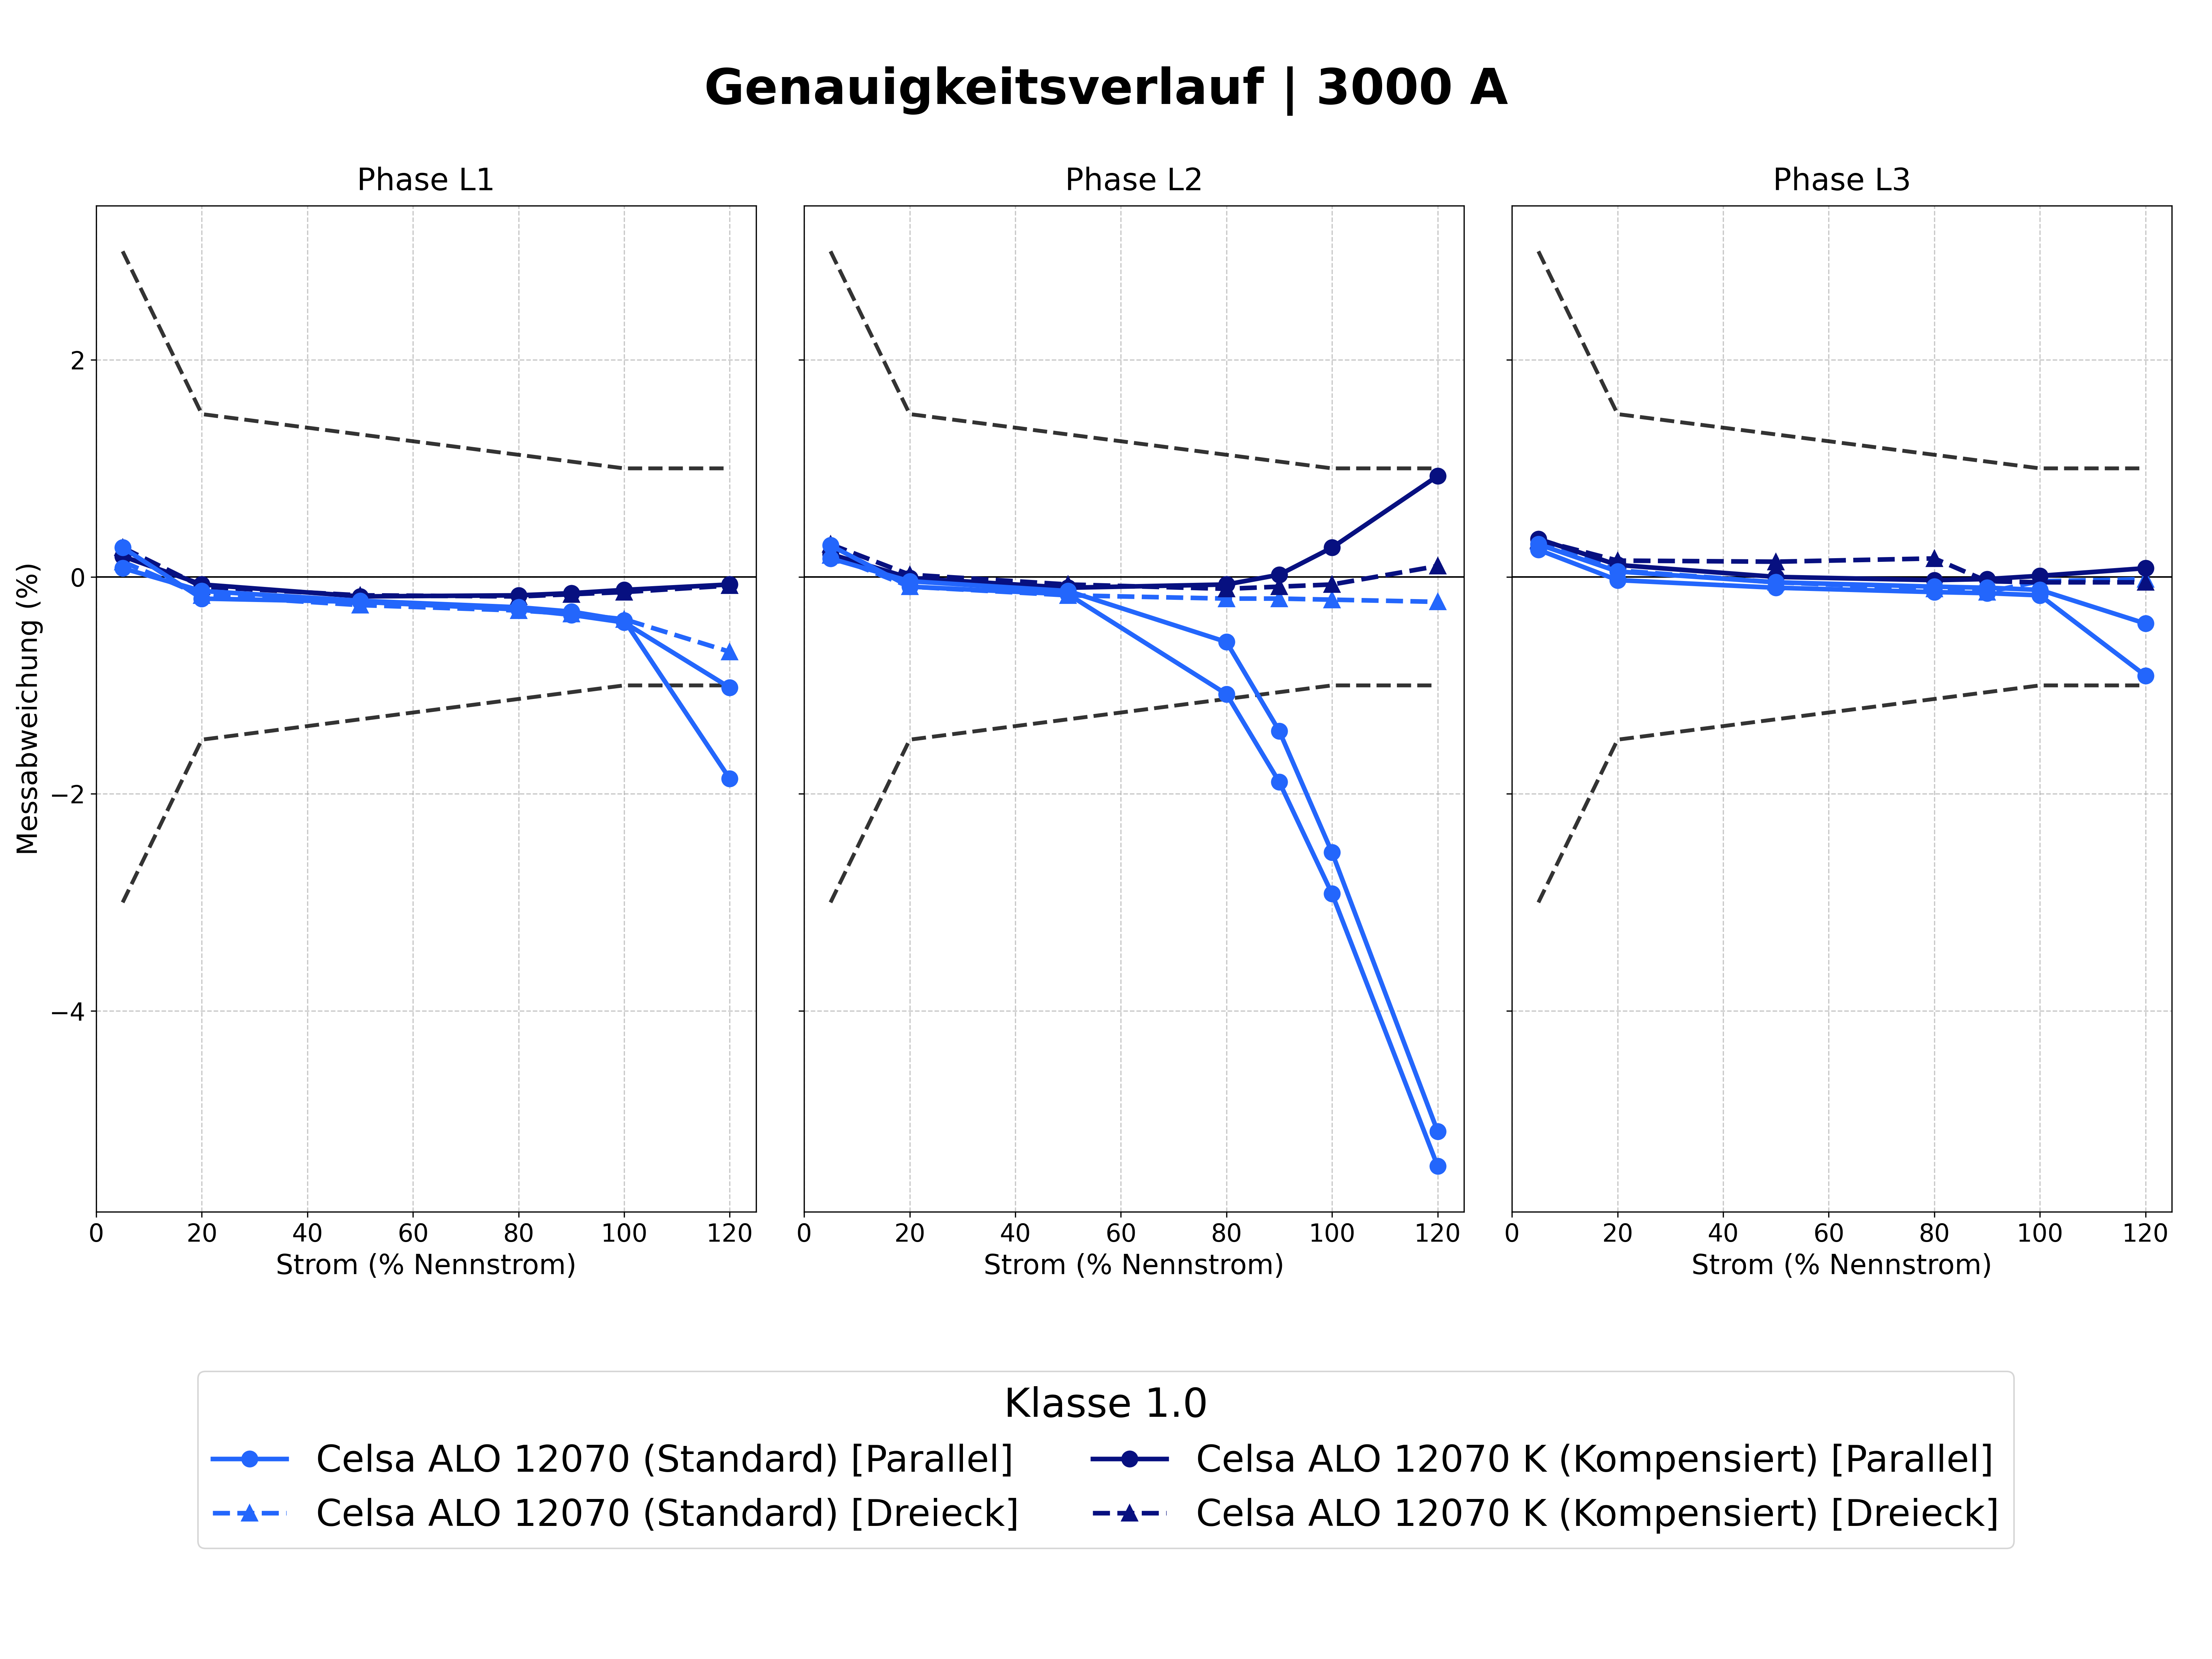
\includegraphics[width=1.0\textwidth]{03_Ressourcen/dia_neu/verlauf/mes_3000A_verlauf.png}
    \caption{Vergleich von Geometrie und Bürdeneinfluss bei \SI{3000}{A}}
    \label{dia:3000A_zusammenfassung}
\end{diagram}

\paragraph{Analyse der Bürdenabhängigkeit}

Da der Standardwandler in der Parallelanordnung erkennbare Sättigungserscheinungen zeigte, wurde in einer vertiefenden Untersuchung analysiert, ob eine Reduktion der sekundären Bürde \gls{sym:RB} diese Effekte kompensieren kann. Hierzu wurden drei Konfigurationen verglichen: die Nennbürde (Referenzlast), der Betrieb ohne Vorwiderstand (Minimallast) und eine asymmetrische Belastung, bei der nur der kritische Leiter L2 entlastet wurde (siehe Tabelle~\ref{tab:buerden_konfigurationen_3000A}).

\begin{table}[H]
    \centering
    \caption{Übersicht der untersuchten Bürdenkonfigurationen bei \SI{3000}{A}}
    \label{tab:buerden_konfigurationen_3000A}
    \small
    \begin{tabular}{l S[table-format=2.2] S[table-format=2.2] S[table-format=2.2] l}
        \toprule
                           & \multicolumn{3}{c}{Bürdenwiderstand \gls{sym:RB} [\unit{\ohm}]} &                                                      \\
        \cmidrule(lr){2-4}
        {Konfiguration}    & {L1}                                                     & {L2} & {L3} & {Ziel der Untersuchung}                \\
        \midrule
        Referenzlast       & 10.80                                                     & 10.80 & 10.80 & Basisvergleich Geometrieeinfluss       \\
        Minimallast        & 0.00                                                      & 0.00  & 0.00  & Bestimmung maximaler Sättigungsgrenze  \\
        Asymmetrische Last & 10.80                                                     & 0.00  & 10.80 & Selektive Entlastung des Mittelleiters \\
        \bottomrule
    \end{tabular}
\end{table}



Abbildung~\ref{dia:3000A_buerde_verlauf} visualisiert die Ergebnisse dieser Variation. Für die Außenleiter L1 und L3 ist kaum eine Abhängigkeit von der Bürde festzustellen, da ihre Abweichungen im Niederstrom- und Nennstrombereich konstant gering bleiben. Anders stellt sich die Situation beim mittleren Leiter L2 dar.

\begin{diagram}[H]
    \centering
    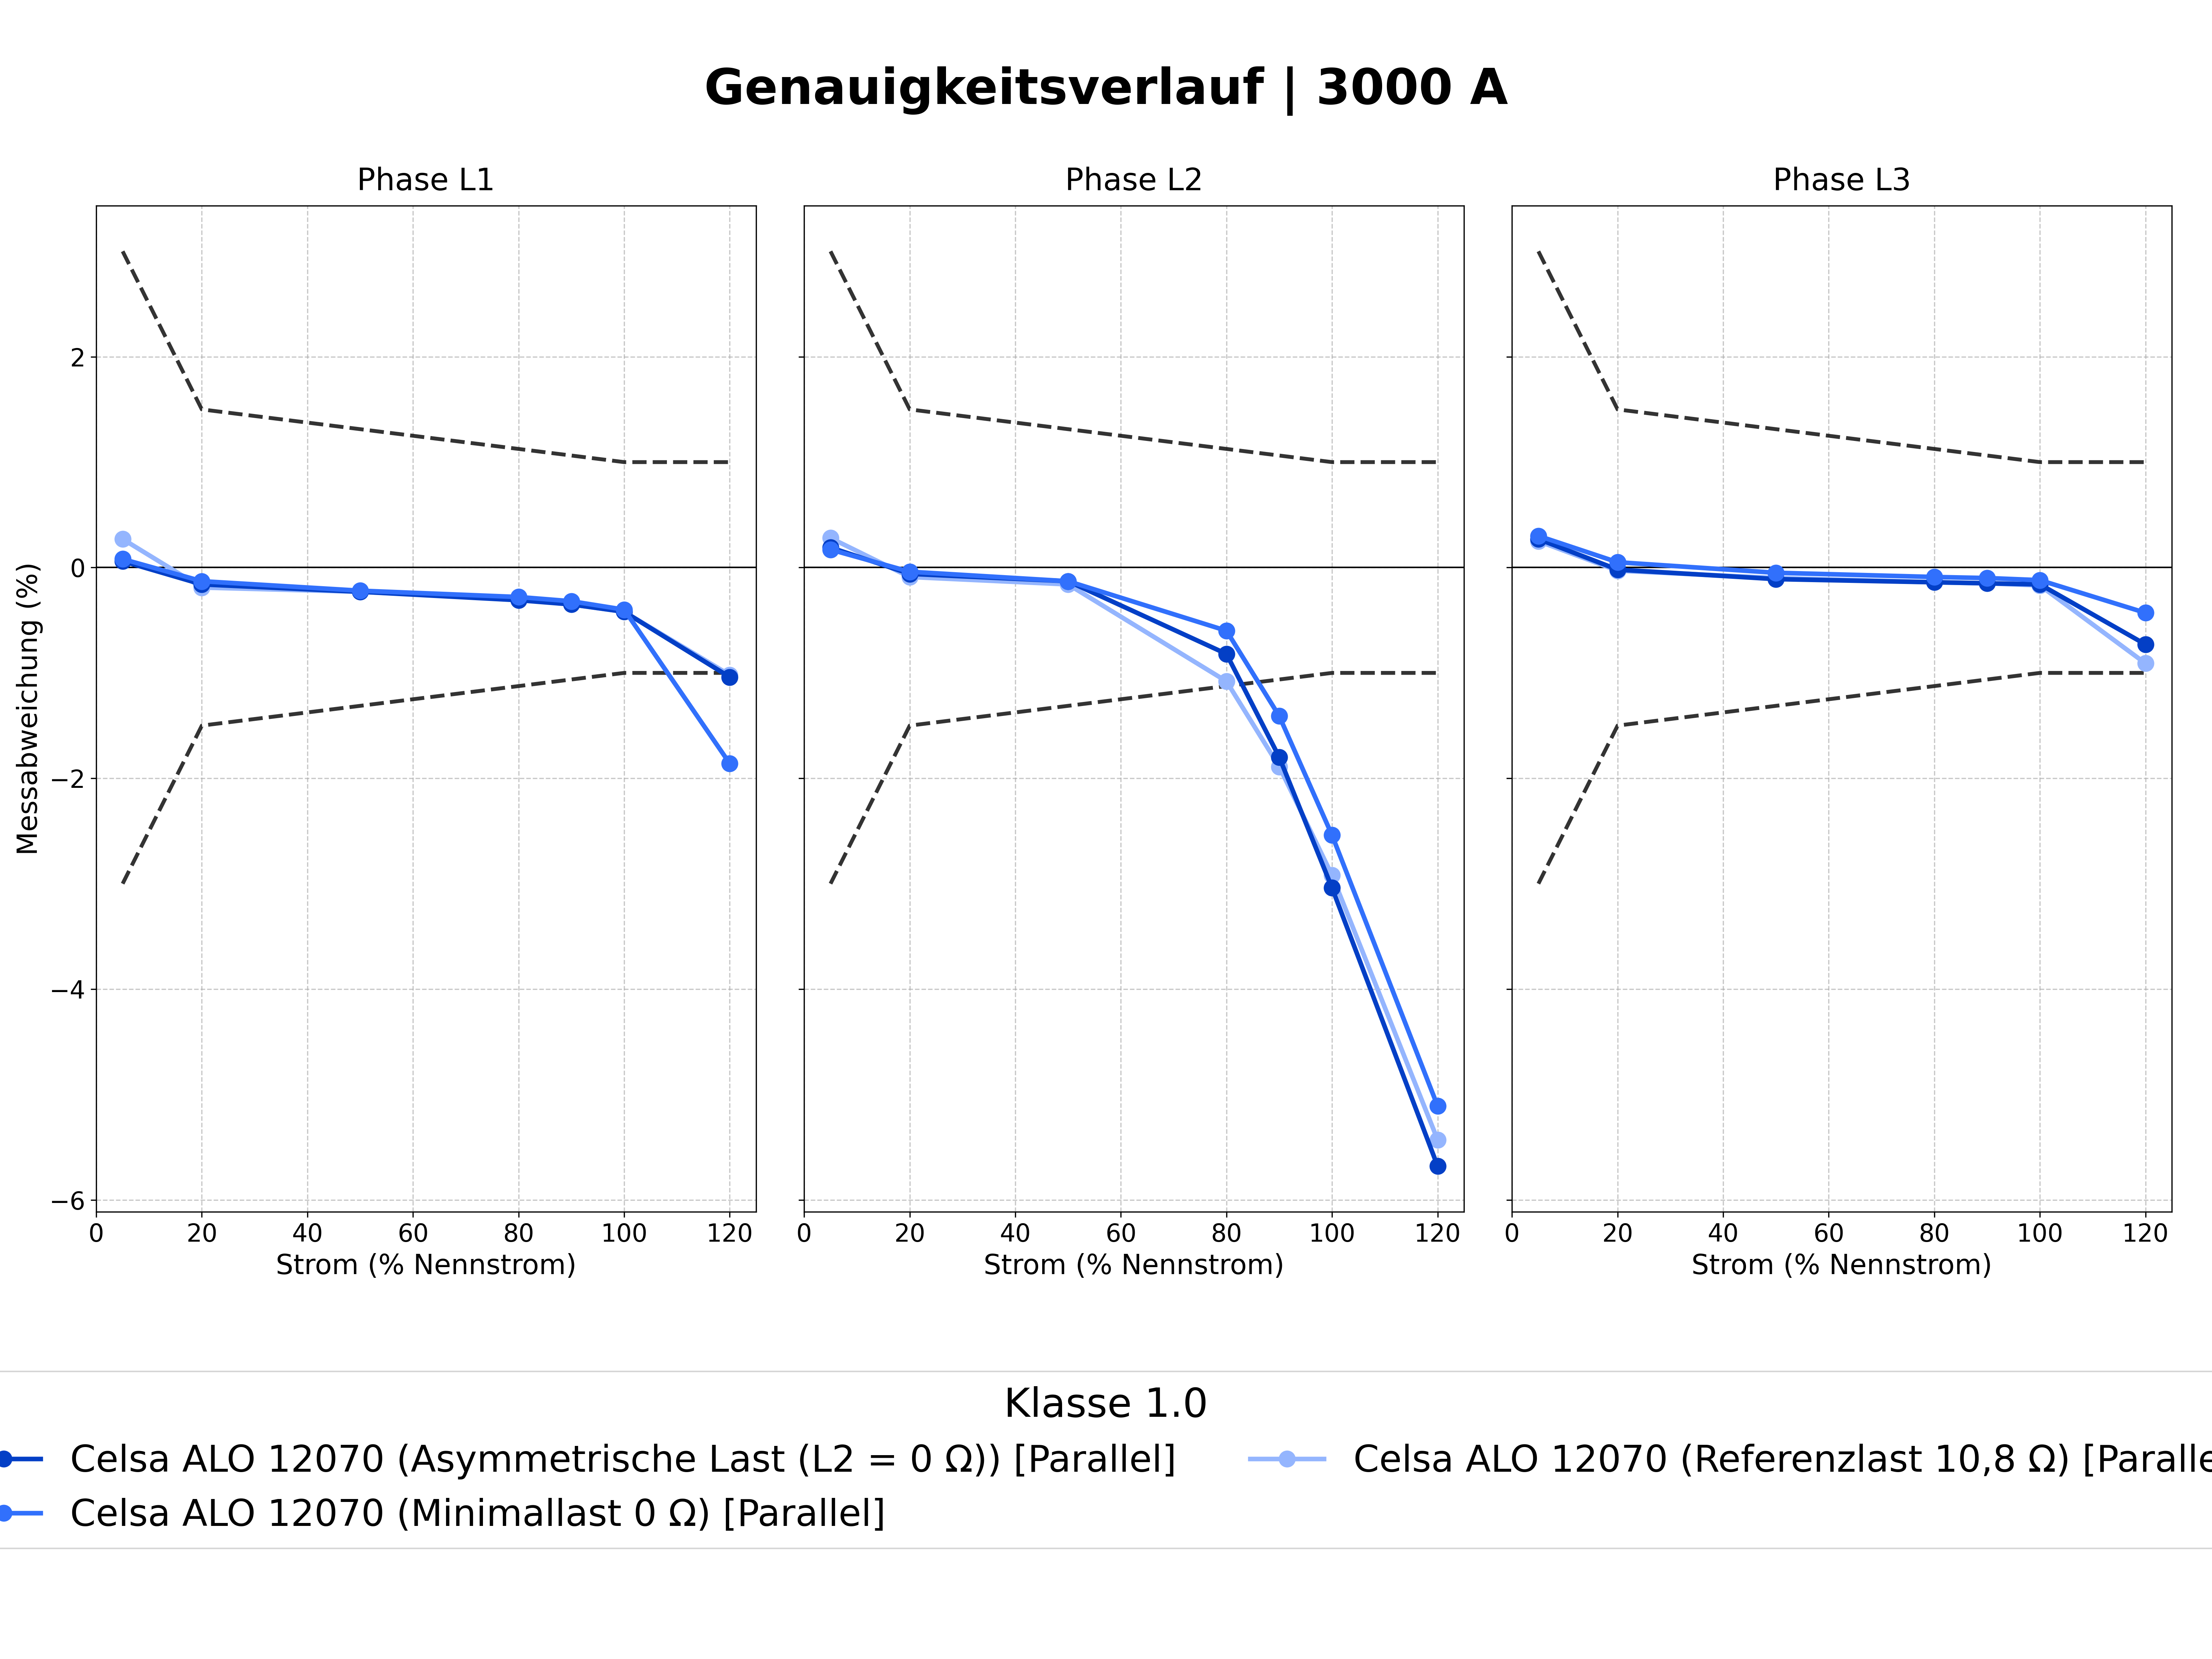
\includegraphics[width=1.0\textwidth]{03_Ressourcen/dia_neu/verlauf/mes_3000A_buerde_verlauf.png}
    \caption{Vergleich der Fehlerkurven bei variabler Bürde \gls{sym:RB} und \SI{3000}{A}}
    \label{dia:3000A_buerde_verlauf}
\end{diagram}

Ein Vergleich zwischen der Referenzlast (Tabelle~\ref{tab:messergebnisse_celsa12070_3000A_alle} im Anhang) und der asymmetrischen Last (Tabelle~\ref{tab:messergebnisse_celsa12070_3000A_asym} im Anhang) zeigt bei L2 ein nahezu identisches Verhalten, da beide Konfigurationen stark sättigen. Während die asymmetrische Last bei \SI{100}{\percent} des Nennstroms \gls{sym:In} bei \num{-3,00}\,\% liegt, weist die Referenzlast mit \num{-2,90}\,\% eine fast gleiche Abweichung auf, was einer Differenz von lediglich \num{0,10}\,\% entspricht. Auch im Überlastbereich bei \SI{120}{\percent} bleiben die Werte vergleichbar, da die asymmetrische Last hier \num{-5,70}\,\% und die Referenzlast \num{-5,40}\,\% erreicht.

Die Konfiguration der Minimallast (Tabelle~\ref{tab:messergebnisse_celsa12070_3000A_min} im Anhang) erweist sich für den kritischen Leiter L2 als die stabilste Variante. Bei \SI{80}{\percent} des Nennstroms liegt der Fehler von L2 hier bei nur \num{-0,60}\,\%, wohingegen die Referenzlast bereits auf \num{-1,10}\,\% abfällt, was eine Verbesserung von rund \num{0,50}\,\% durch die minimale Bürde bedeutet. Dennoch reicht auch die Minimallast nicht aus, um den Standardwandler in der Parallelanordnung bei Nennstrom \gls{sym:In} in die Genauigkeitsklasse \num{1} zurückzuführen (\num{-2,50}\,\% Abweichung).

Der Performance-Index in Abbildung~\ref{dia:3000A_performance_buerde} fasst die Ergebnisse zusammen. Zwar erzielt die Messung mit der Minimallast über alle Strombereiche hinweg die besten Ergebnisse, doch zeigt der Vergleich mit dem vorangegangenen Abschnitt, dass die Wahl der Wandlertechnologie (Kompensation) und der Geometrie (Dreieck) einen weitaus größeren Einfluss auf die Messgüte hat als die Optimierung der Bürde. Die Reduktion des Widerstands zögert die Sättigung physikalisch bedingt zwar hinaus, kann die systembedingten Schwächen der Parallelanordnung bei Standardwandlern jedoch nicht vollständig kompensieren.

\begin{diagram}[H]
    \centering
    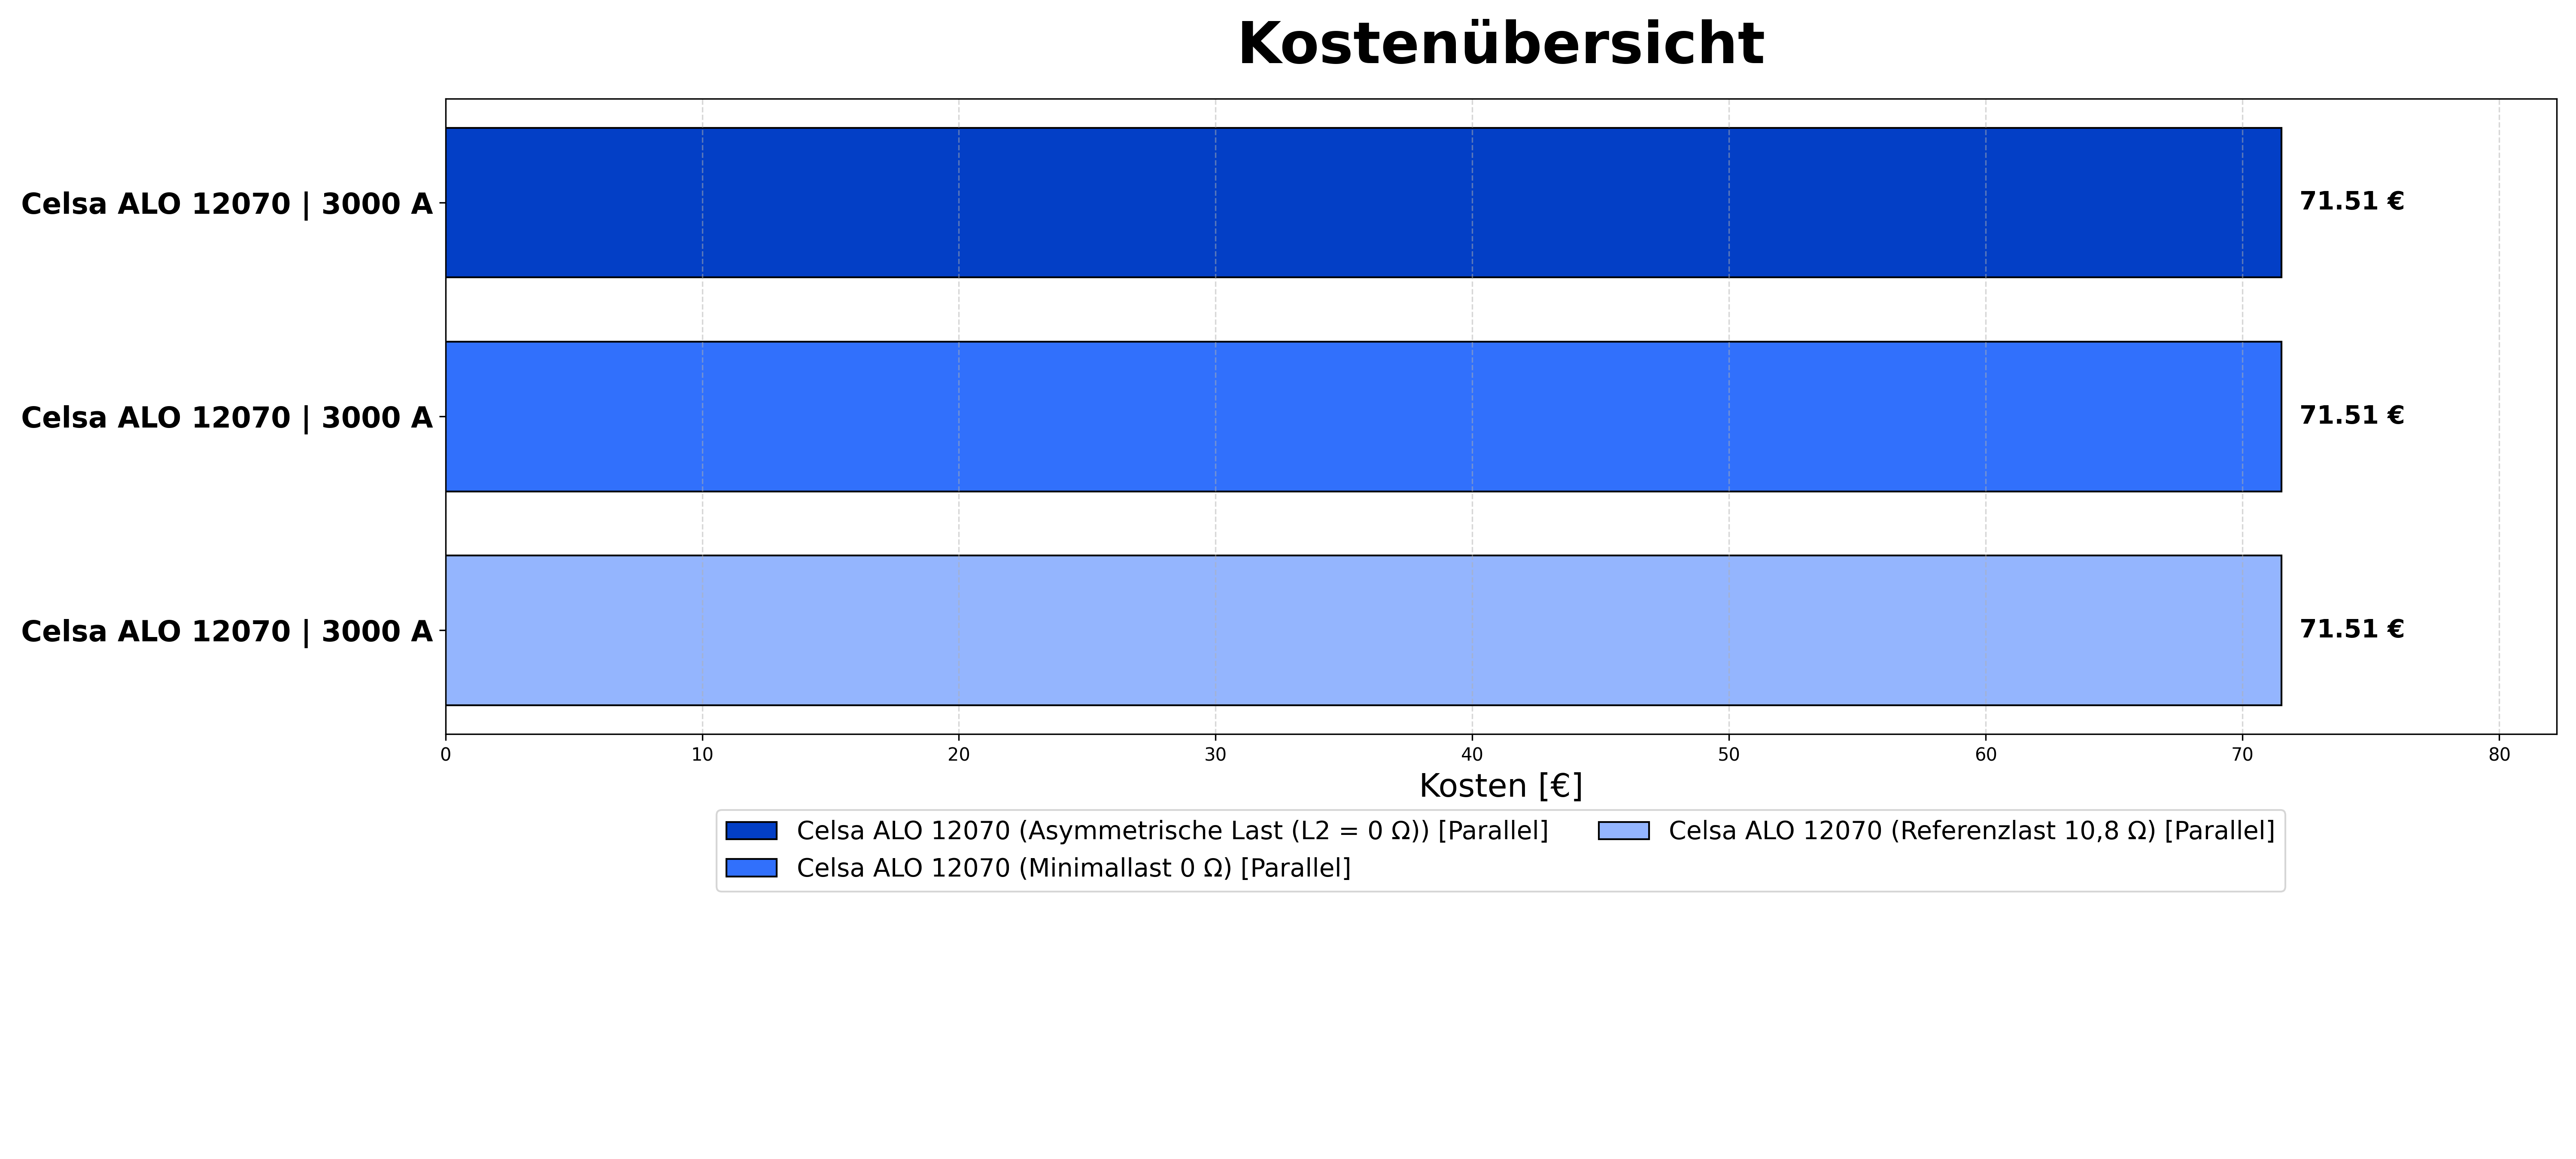
\includegraphics[width=1.0\textwidth]{03_Ressourcen/dia_neu/kosten_horizontal/mes_3000A_buerde_kosten_horizontal.png}
    \caption{Ranking der Konfigurationen basierend auf dem Performance-Index}
    \label{dia:3000A_performance_buerde}
\end{diagram}


\subsubsection{Skalierung der Geometrieeffekte bei \SI{4000}{A}}
\label{sec:analyse_messreihe_4000A}

Für diese Messreihe wurde der Phasenmittenabstand gemäß Tabelle~\ref{tab:schienen_konfiguration} auf den für diese Stromstärke üblichen Wert vergrößert. Mit der Steigerung des Nennstroms \gls{sym:In} auf \SI{4000}{A} rückt die Reproduzierbarkeit der geometrischen Einflüsse bei gleicher Wandlerbauform in den Vordergrund. Betrachtet werden erneut die Typen der Reihe \textit{Celsa~ALO~12070} in Standardausführung sowie in der kompensierten Variante \textit{Celsa~ALO~12070~K}. Die Ergebnisse dienen dazu, das Verhalten der Wandler bei weiter steigender Sättigung ohne den Einfluss variabler Bürdenwiderstände zu verifizieren.



Abbildung~\ref{dia:4000A_zusammenfassung} skizziert einen Verlauf, der qualitativ stark den Beobachtungen aus Abschnitt \ref{sec:analyse_messreihe_3000A} ähnelt. Sowohl in der Parallelanordnung als auch in der Dreieckskonfiguration stößt der Standardwandler \textit{Celsa~ALO~12070} hier an seine physikalischen Leistungsgrenzen, wenngleich zu unterschiedlichen Zeitpunkten.

\begin{diagram}[H]
    \centering
    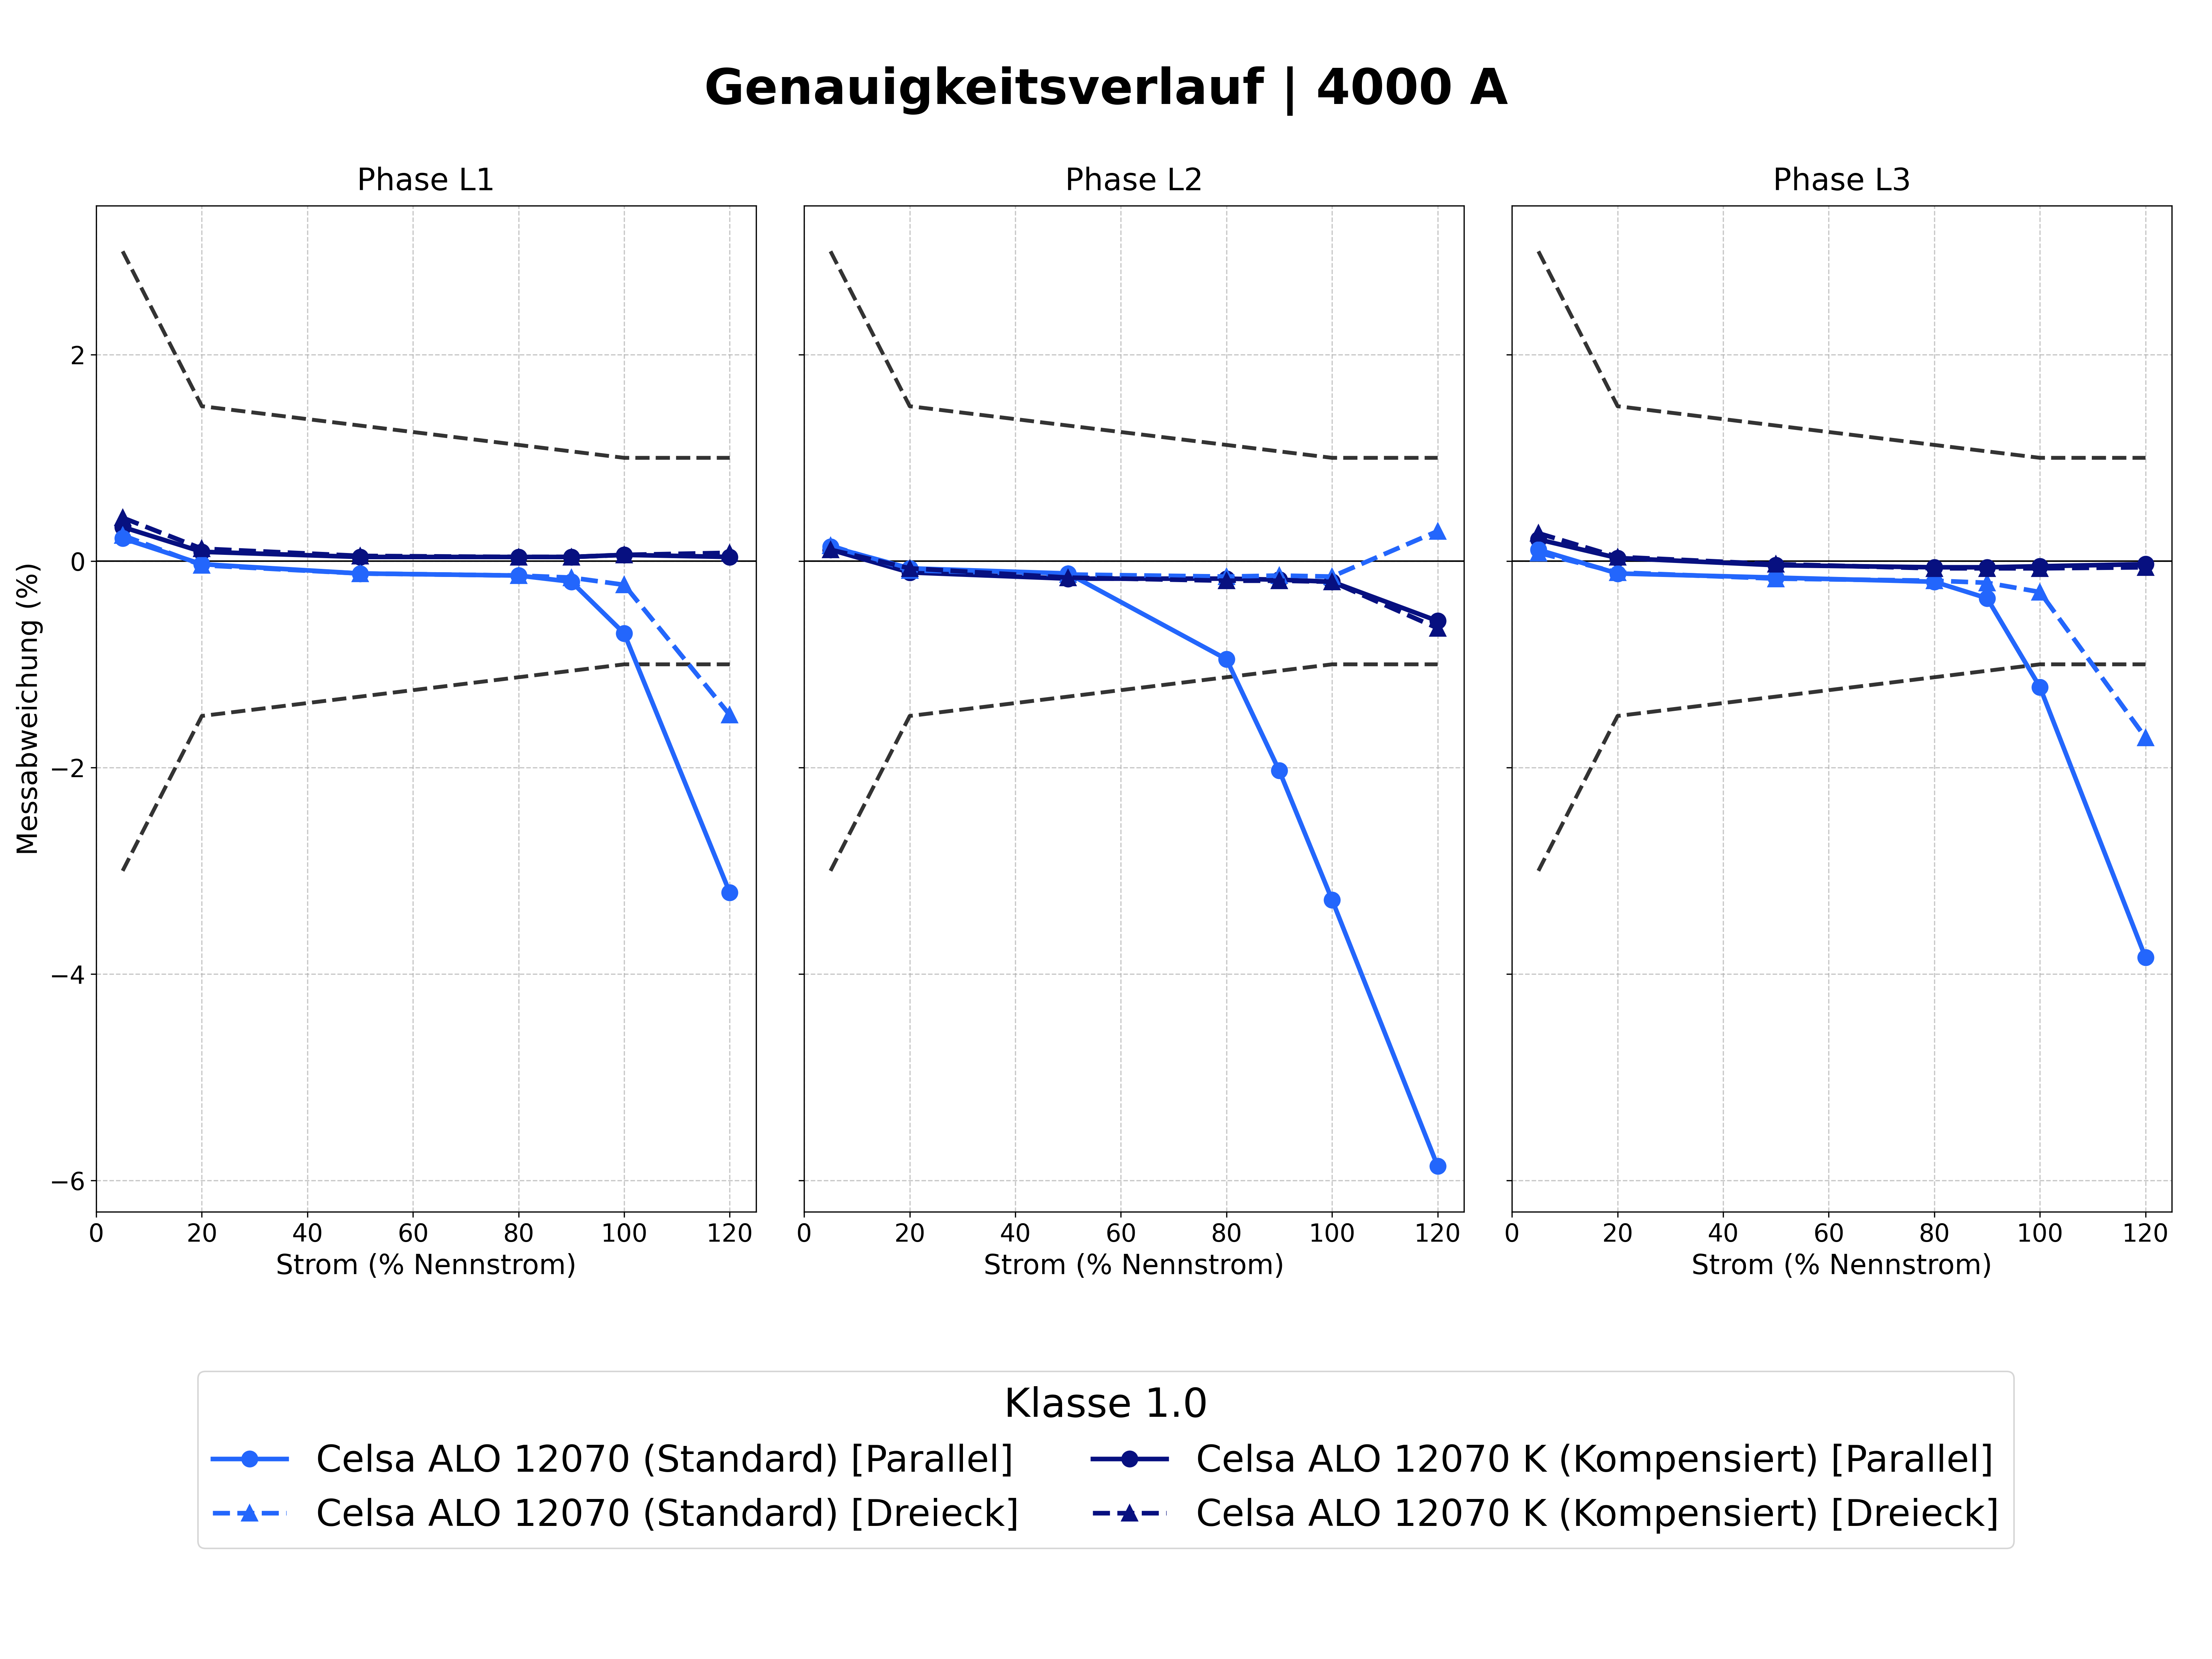
\includegraphics[width=1.0\textwidth]{03_Ressourcen/dia_neu/verlauf/mes_4000A_verlauf.png}
    \caption{Zusammenfassender Vergleich der Leitergeometrien bei \SI{4000}{A}}
    \label{dia:4000A_zusammenfassung}
\end{diagram}

Besonders augenfällig wird dies in der Parallelanordnung. Wie die Werte in Tabelle~\ref{tab:messergebnisse_celsa12070_4000A_alle} im Anhang belegen, bricht die Genauigkeit ab \SI{80}{\percent} des Nennstroms \gls{sym:In} drastisch ein. Bei \SI{3200}{A} weist der mittlere Leiter L2 bereits eine Übersetzungsmessabweichung \gls{sym:epsilon} von \num{-0,90}\,\% auf und verlässt bei weiterer Lasterhöhung den Toleranzbereich der Genauigkeitsklasse \num{1}. Bei Nennstrom (\SI{4000}{A}) liegt der Fehler bei \num{-3,30}\,\%. 

Dieser Einbruch bei etwa \SI{3200}{A} korreliert signifikant mit den Sättigungseffekten der \SI{3000}{A}-Messreihe, was darauf hindeutet, dass die physikalische Sättigungsgrenze des Eisenkerns in der Parallelgeometrie in diesem Lastbereich liegt. Dieses Verhalten spiegelt die Problematik wider, welche bereits beim Typ \textit{Celsa~ALO~10030} bei \SI{2000}{A} und \SI{2500}{A} beobachtet wurde, wo die Parallelanordnung ebenfalls zu einer vorzeitigen Sättigung durch Fremdfeldeinflüsse führte.



Die Umstellung auf die Dreieckskonfiguration bewirkt bei Nennstrom eine deutliche Verbesserung. Die Abweichung \gls{sym:epsilon} der Phase L2 reduziert sich hierbei von \num{-3,30}\,\% in der Parallelanordnung auf \num{-0,15}\,\% in der Dreieckskonfiguration, womit die Genauigkeitsklasse \num{1} bei \SI{100}{\percent} Last wieder eingehalten wird. Allerdings zeigt sich im Überlastbereich bei \SI{120}{\percent}, dass auch die Dreiecksanordnung die magnetische Sättigung nicht vollständig verhindern kann, da hier die Außenleiter L1 und L3 mit \num{-1,50}\,\% beziehungsweise \num{-1,70}\,\% die normativen Klassengrenzen überschreiten.




\subsection{Ökonomische Evaluation und Technologie-Ranking}
\label{sec:oekonomische_evaluation}

In diesem Abschnitt werden die technischen Messergebnisse in Relation zu den Anschaffungskosten gesetzt, um eine fundierte ökonomische Bewertung der verschiedenen Wandlertechnologien vorzunehmen. Hierfür wurde ein \textit{Performance-Score} ermittelt, der sich aus der gewichteten Summe der gemittelten Betragsabweichung \gls{sym:epsilon} und dem Marktpreis zusammensetzt. Ziel ist die Identifikation des optimalen Preis-Leistungs-Verhältnisses für den jeweiligen industriellen Anwendungsfall.



% --- Cluster 1: Standardbereich ---
\subsubsection{Wirtschaftlichkeit im Nennstrombereich (\SI{2000}{A} bis \SI{2500}{A})}

Im Bereich zwischen \SI{2000}{A} und \SI{2500}{A} werden die unterschiedlichen Wandlertechnologien unmittelbar vergleichbar, da alle untersuchten Typen ihre Messaufgabe grundsätzlich innerhalb oder nahe der geforderten Genauigkeitsklasse \num{1} erfüllen. Der wirtschaftliche Vergleich stellt somit weniger eine Frage der grundsätzlichen Funktionstüchtigkeit dar, sondern vielmehr der Effizienz des eingesetzten technischen Aufwands.

\begin{diagram}[H]
    \centering
    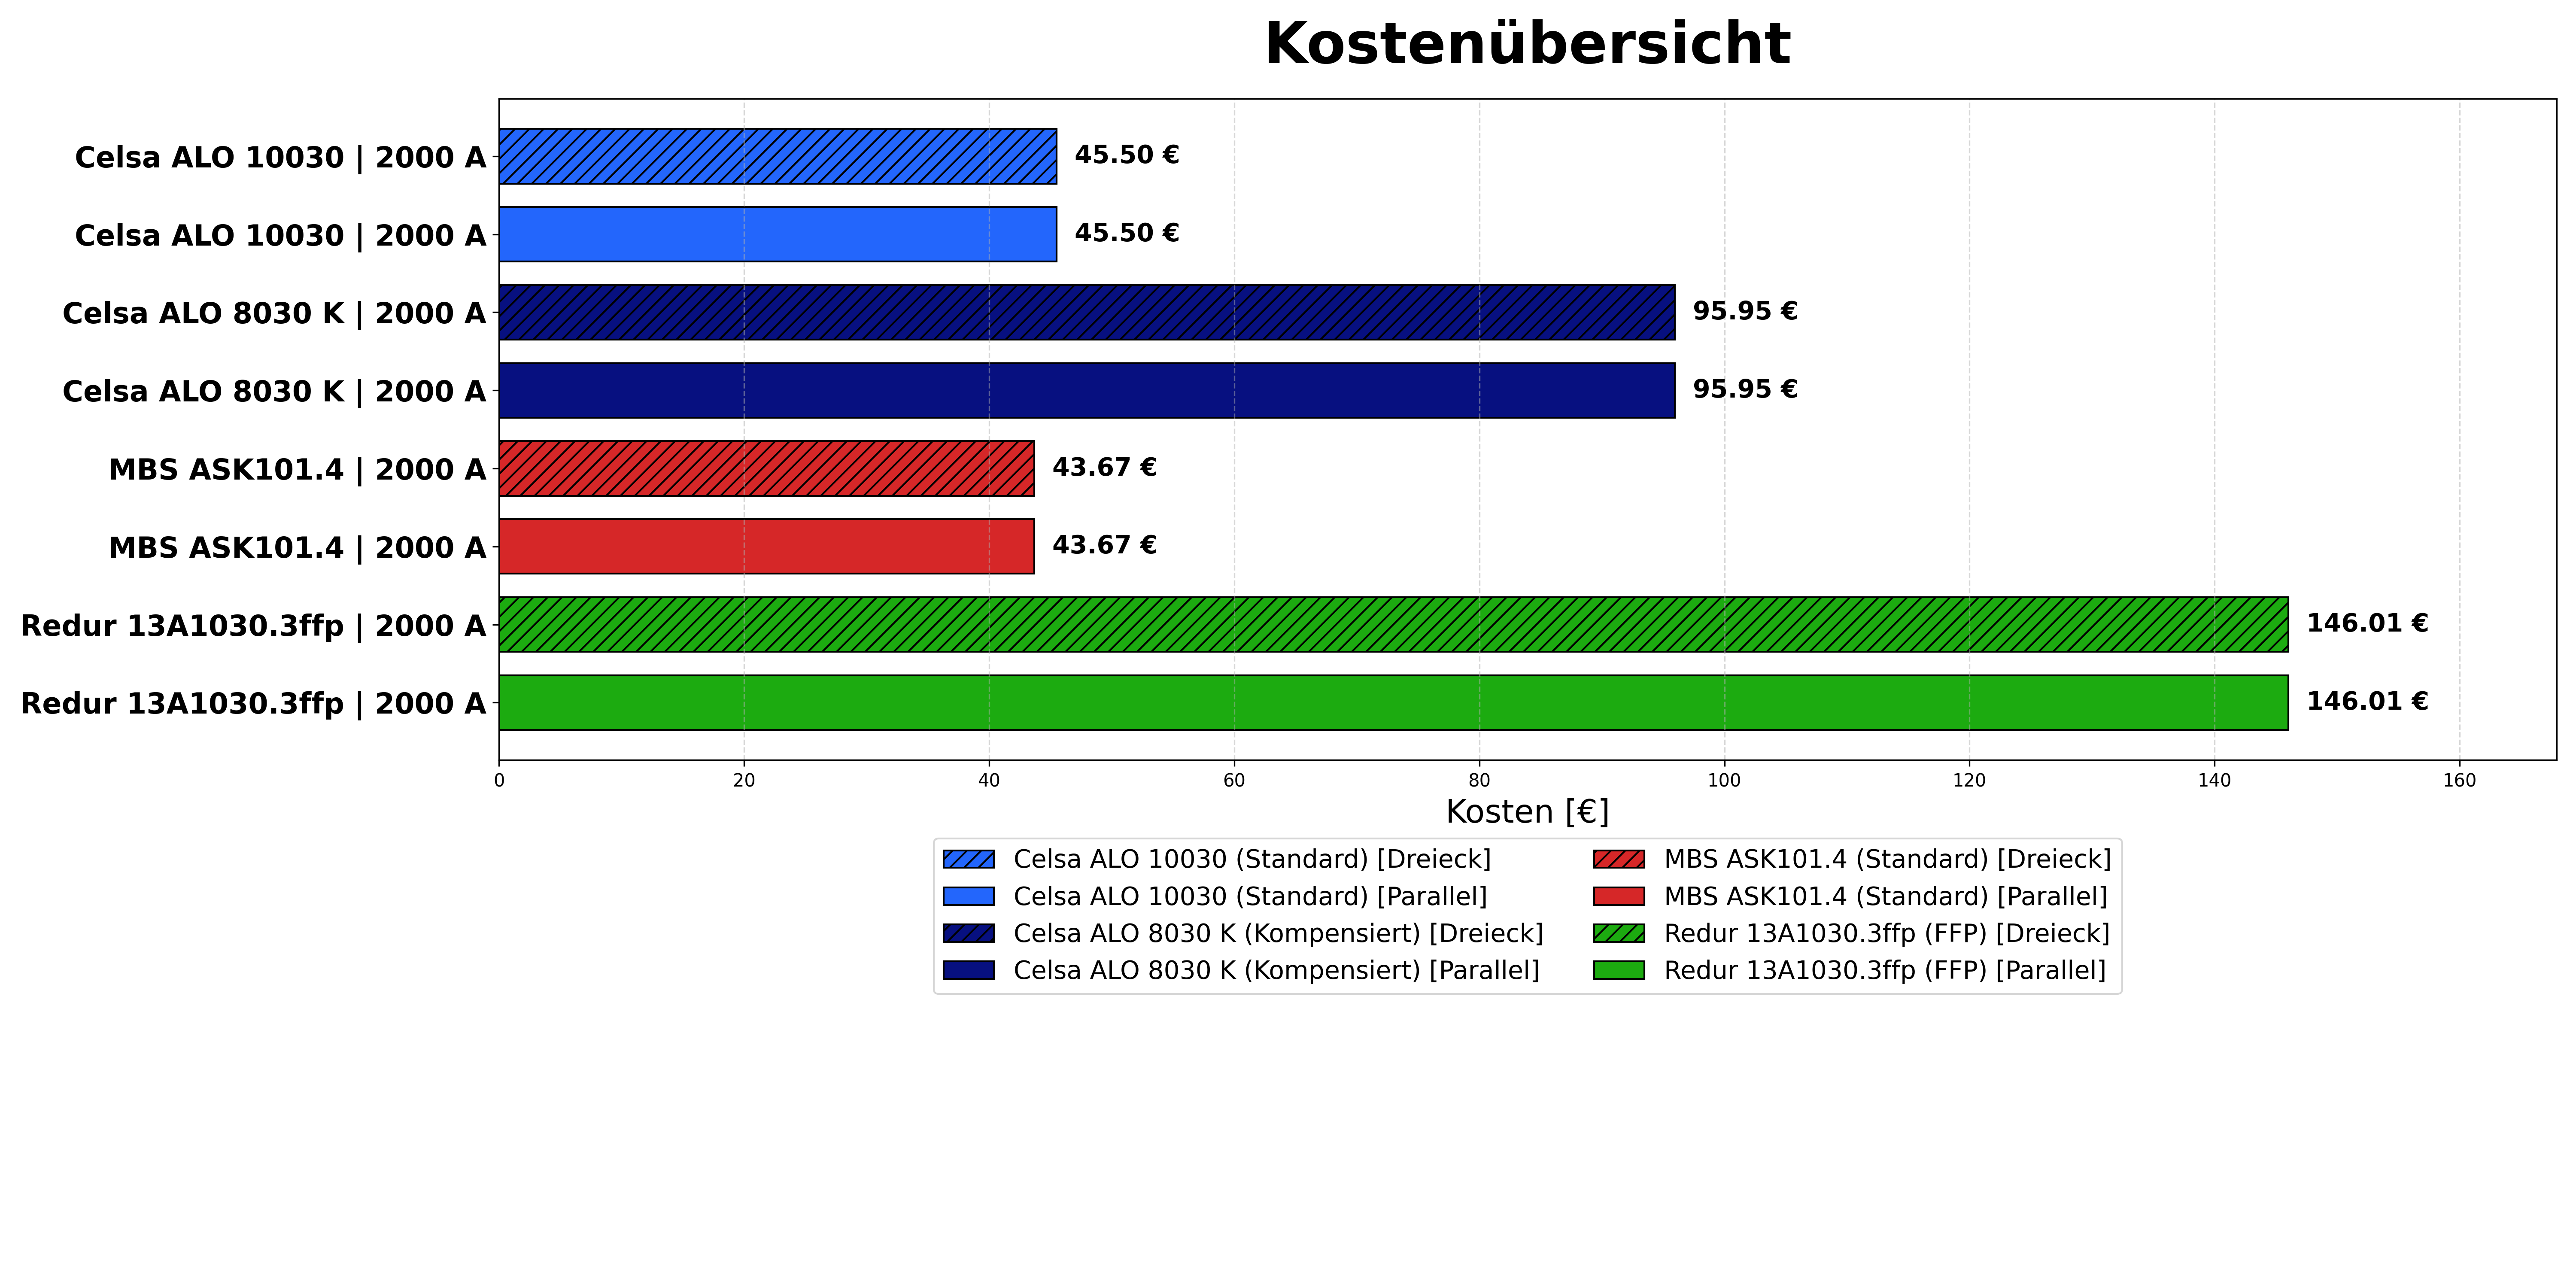
\includegraphics[width=0.9\textwidth]{03_Ressourcen/dia_neu/kosten_horizontal/mes_2000A_kosten_horizontal.png}
    \caption{Wirtschaftliches Ranking der Wandlertechnologien bei \SI{2000}{A}}
    \label{dia:2000A_ranking_plot}
\end{diagram}

Als preisliche Referenz fungieren die Standardwandler ohne zusätzliche Kompensations- oder Abschirmmaßnahmen, exemplarisch vertreten durch den \textit{Celsa~ALO~10030} sowie den \textit{MBS~ASK101.4}. Diese Modelle weisen die geringsten Anschaffungskosten auf, zeigen jedoch — insbesondere in der Parallelanordnung — eine erhöhte Empfindlichkeit gegenüber externen Magnetfeldern. Dies schlägt sich in einem erhöhten Fehleranteil im Performance-Score nieder, wodurch der rein preisliche Vorteil teilweise relativiert wird (siehe Abbildung~\ref{dia:2000A_ranking_plot}).

Demgegenüber stehen die kompensierten Wandler von \textit{Celsa} (\textit{ALO~8030K} bzw. \textit{ALO~10050~K}), die durch ihre zusätzliche Wicklung eine deutlich höhere Messstabilität erreichen. Die geringeren Fehleranteile führen trotz höherer Anschaffungskosten zu konkurrenzfähigen Performance-Scores, insbesondere bei \SI{2500}{A} (siehe Abbildung~\ref{dia:2500A_ranking_plot}). In diesem Strombereich rechtfertigt der technische Mehraufwand somit erstmals ökonomisch den höheren Preis.

\begin{diagram}[H]
    \centering
    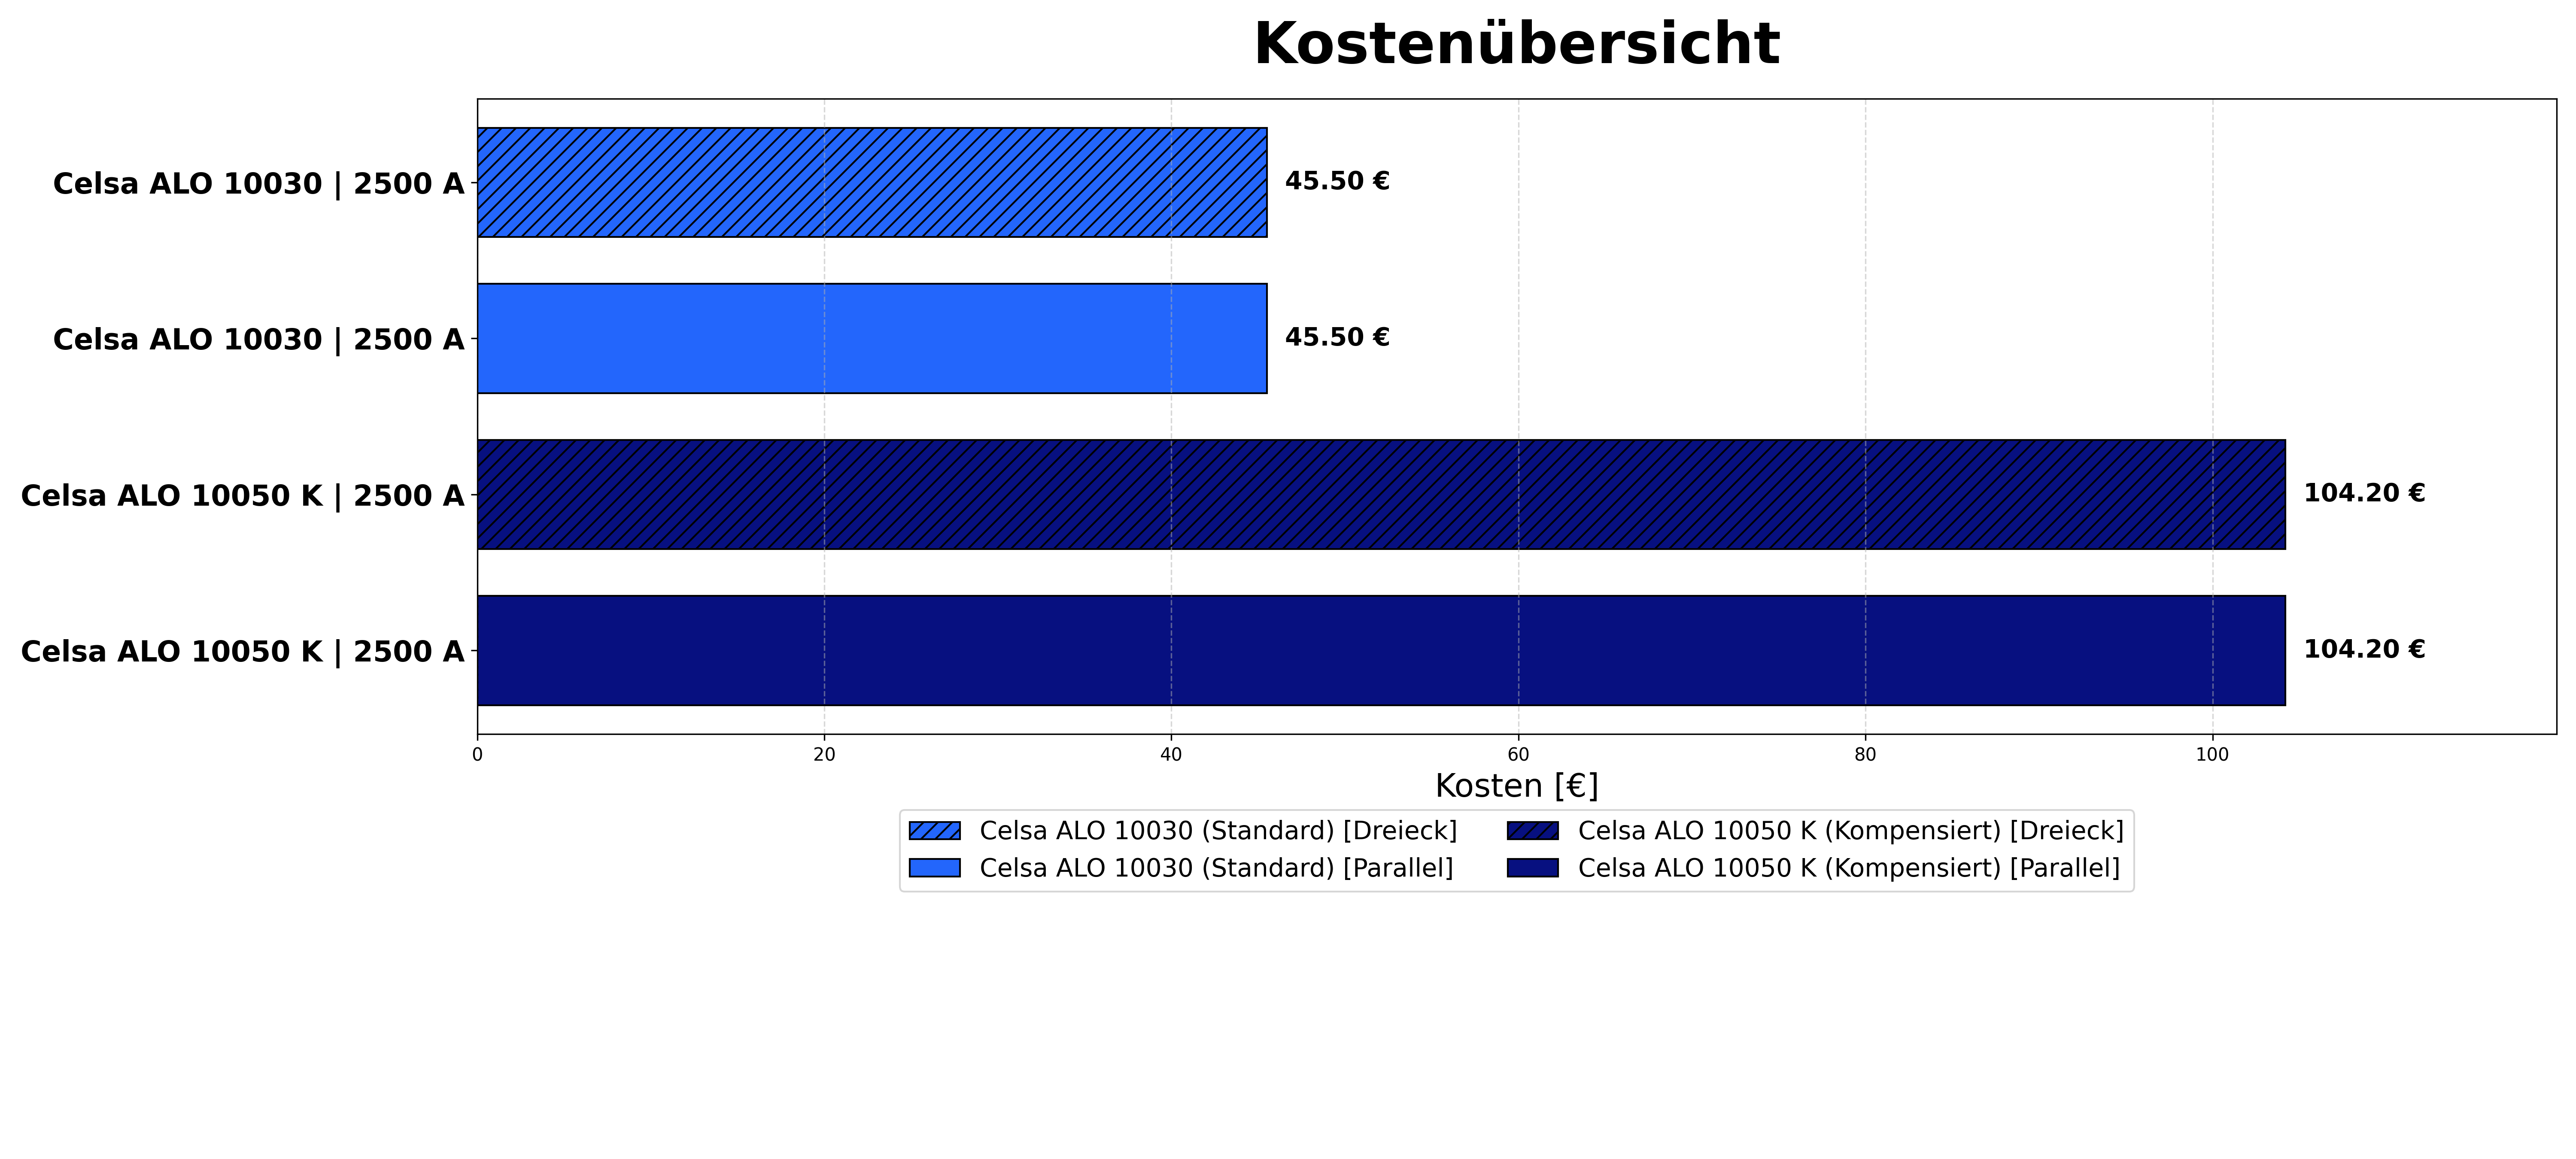
\includegraphics[width=0.9\textwidth]{03_Ressourcen/dia_neu/kosten_horizontal/mes_2500A_kosten_horizontal.png}
    \caption{Wirtschaftliches Ranking der Wandlertechnologien bei \SI{2500}{A}}
    \label{dia:2500A_ranking_plot}
\end{diagram}



Eine weitere Technologiestufe stellen Wandler mit Fremdfeldprotektoren dar, vertreten durch die \textit{Redur-Modelle}. Diese zeichnen sich durch eine hohe geometrische Robustheit aus und zeigen selbst in ungünstigen Leiteranordnungen stabile Messwerte. Ökonomisch bewegen sie sich jedoch aufgrund der hohen Anschaffungskosten nur im oberen Mittelfeld, da der Zugewinn an Messgenauigkeit im Nennstrombereich bis \SI{2500}{A} begrenzt bleibt. 

Für den Nennstromfall \SI{2000}{A} ist zudem die Parallelanordnung des \textit{Redur~13A1030.3ffp} hervorzuheben. Die Fremdfeldprotektoren (\gls{ffp}) reduzieren in dieser Konfiguration die Messabweichungen insbesondere im Nenn- und Überlastbereich deutlich. Ein zusätzlicher Vorteil der Protektor-Technologie besteht darin, dass Abschirmkörper prinzipiell auch als nachrüstbare Maßnahme in bestehenden Anlagen eingesetzt werden können. Damit eröffnet sich eine wirtschaftlich interessante Option zur Verbesserung der Messgenauigkeit, ohne den Stromwandler vollständig ersetzen zu müssen \cite{pdf-Patent_Abschirmung-Redur}.

Ist die Realisierung einer Dreieckskonfiguration aus konstruktiven oder normativen Gründen nicht möglich, muss die Auswahl auf die Parallelanordnung beschränkt werden. In diesem Fall verlieren feldempfindliche Standardwandler ihren Kostenvorteil, da erhöhte Messabweichungen den Performance-Score dominieren. Für den betrachteten Datensatz bei \SI{2000}{A} erzielt der \textit{MBS~ASK101.4} in Parallelanordnung den geringsten Performance-Index und stellt damit die wirtschaftlich günstigste Lösung dar. Bei \SI{2500}{A} verschiebt sich das Optimum hingegen zugunsten des kompensierten \textit{Celsa~ALO~10050~K}, der auch ohne geometrische Optimierung stabile Messwerte liefert.

% --- Cluster 2: Hochstrombereich ---
\subsubsection{Verschiebung der Kosteneffizienz bei Hochstrom (\SI{3000}{A} bis \SI{4000}{A})}

Die Messreihen bei \SI{3000}{A} und \SI{4000}{A} zeigen exemplarisch, wie sich die Wirtschaftlichkeit bei gleicher Wandlerbauform mit steigender Stromstärke verschiebt. In beiden Fällen werden die Baureihe \textit{Celsa~ALO~12070} in Standardausführung sowie die kompensierte Variante \textit{Celsa~ALO~12070~K} gegenübergestellt.

\begin{diagram}[H]
    \centering
    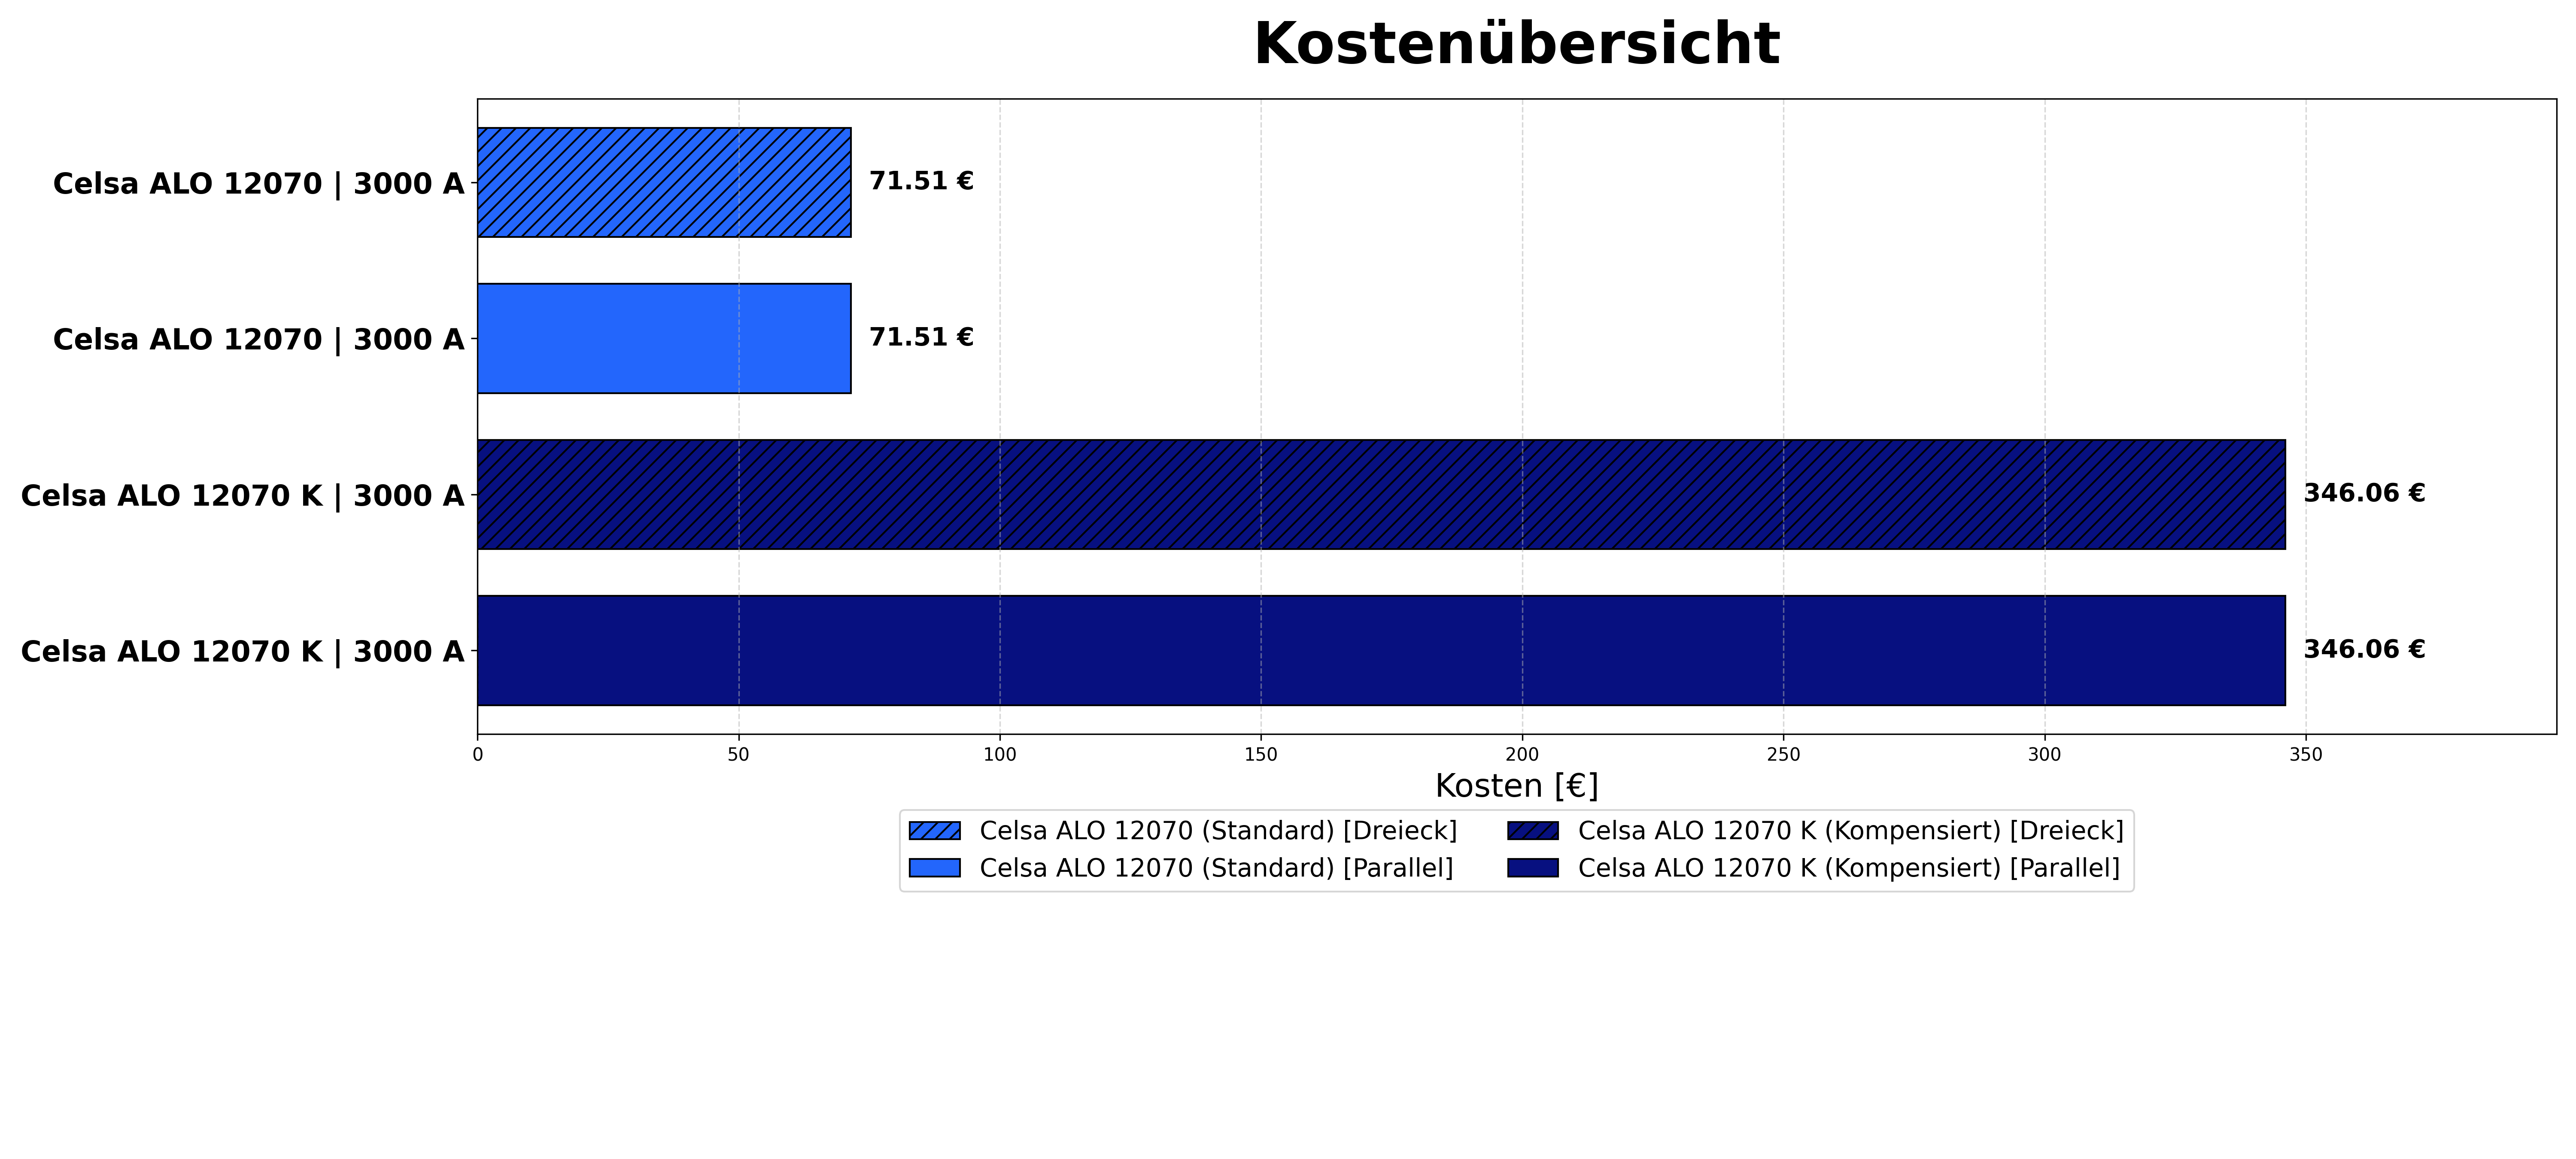
\includegraphics[width=0.9\textwidth]{03_Ressourcen/dia_neu/kosten_horizontal/mes_3000A_kosten_horizontal.png}
    \caption{Wirtschaftliches Ranking der Wandlertechnologien bei \SI{3000}{A}}
    \label{dia:3000A_ranking_plot}
\end{diagram}



Bei \SI{3000}{A} (Abbildung~\ref{dia:3000A_ranking_plot}) wird der Performance-Score bereits massiv durch den Messfehler beeinflusst. Insbesondere in der Parallelanordnung verliert der nicht kompensierte Standardwandler seinen Kostenvorteil. Die kompensierte Ausführung erreicht dadurch trotz höherer Anschaffungskosten ein günstigeres Preis-Leistungs-Verhältnis. Bei \SI{4000}{A} (Abbildung~\ref{dia:4000A_ranking_plot}) verstärkt sich dieser Effekt drastisch: Mit steigender Strombeanspruchung wächst der Abstand im Ranking, da die Sättigungseffekte bei Standardwandlern überproportional zunehmen.

\begin{diagram}[H]
    \centering
    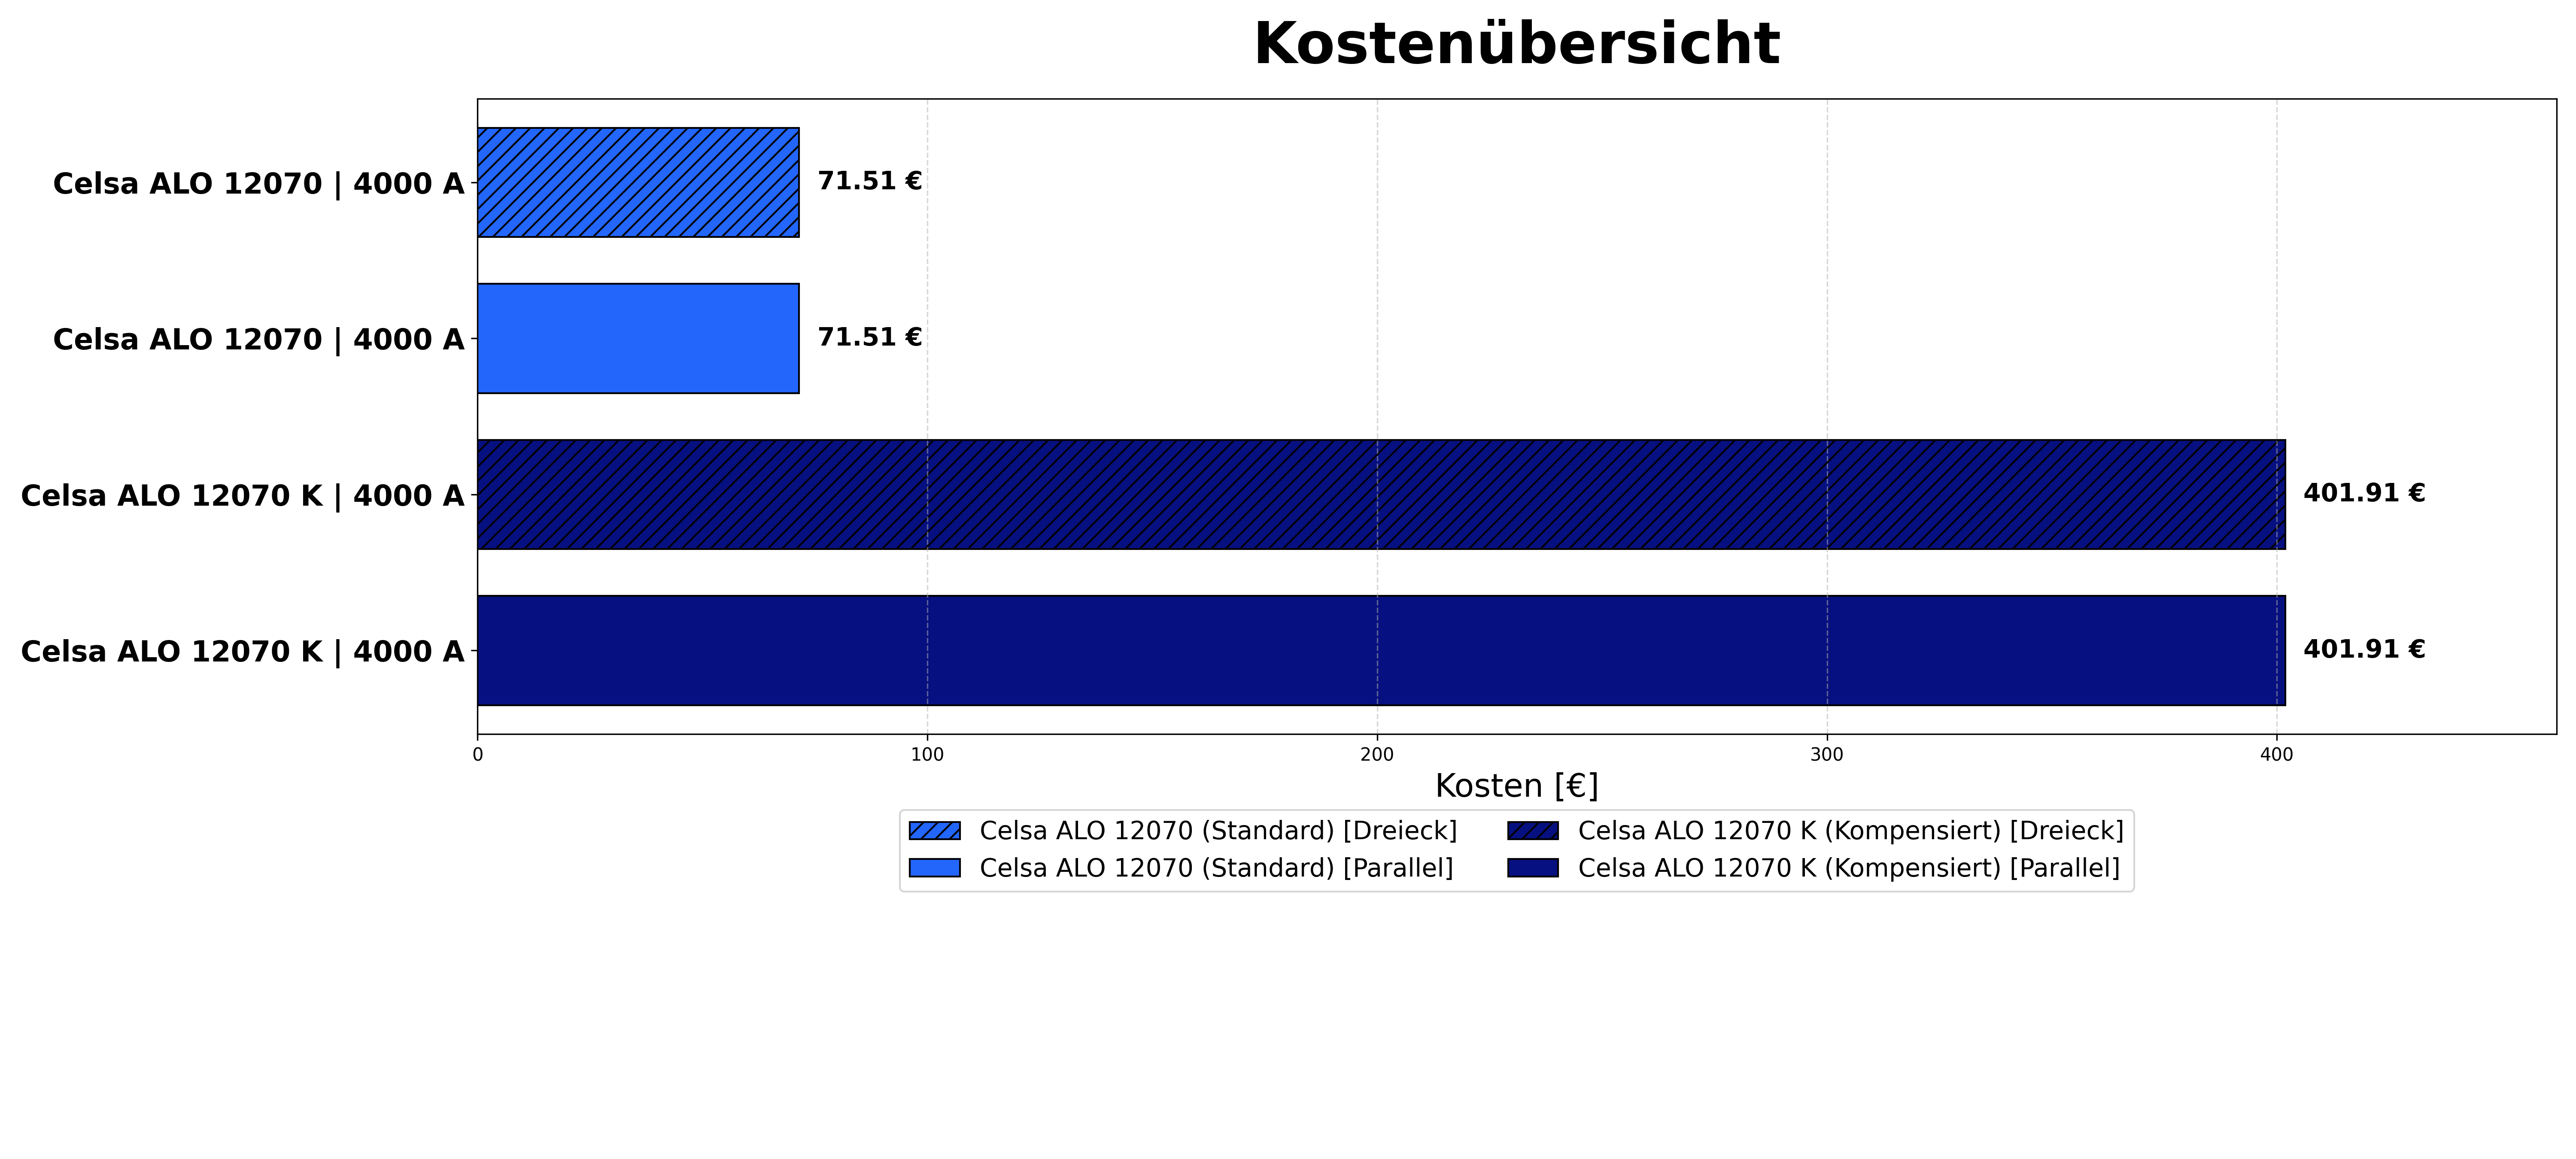
\includegraphics[width=0.9\textwidth]{03_Ressourcen/dia_neu/kosten_horizontal/mes_4000A_kosten_horizontal.png}
    \caption{Wirtschaftliches Ranking der Wandlertechnologien bei \SI{4000}{A}}
    \label{dia:4000A_ranking_plot}
\end{diagram}

Parallel dazu zeigt sich der Einfluss der Leitergeometrie als eigenständiger wirtschaftlicher Hebel. Die Dreieckskonfiguration senkt die Messabweichungen \gls{sym:epsilon} und verbessert damit den Performance-Score über alle Technologieklassen hinweg. Eine geometrische Optimierung verbessert die Wirtschaftlichkeit somit deutlich effektiver als eine reine Bürdenanpassung.


